\chapter{仿真结果}
\label{sec:results}

在本章中,我们展示我们的流体仿真方法在不同领域中的应用。其中,通过第~\ref{sec:siga21} 章中的方法得到的结果均于一个14核Intel CPU、128 GB内存、NVIDIA RTX 3090的工作站上仿真获得;通过第~\ref{sec:sig23} 章中的方法得到的结果均于一个20核Intel CPU、128 GB内存、NVIDIA A100 GPU的工作站上仿真获得。

\section{面向视觉动画的仿真结果}
下面我们首先展示一系列面向视觉动画的仿真结果。首先使用第~\ref{sec:siga21} 章描述的方法,我们对一系列的复杂几何进行单向与双向流固耦合仿真,以显示我们的方法处理不同类型物体的能力。我们还展示了一些可交互的仿真与离线的高分辨率大规模仿真,包括对一些实际物理现象的复现。

结果中的展示的烟雾均使用染色粒子对仿真产生的流场进行被动追踪生成,这些粒子最终会被转换成OpenVDB文件~\cite{Museth-2013},并使用RedShift渲染器~\cite{redshift} 进行渲染。

\begin{figure}[!htbp]
  \centering
    \includegraphics[width=0.99\columnwidth]{figures/result_tube.png}
  \bicaption[旋转的薄圆柱面]{旋转的薄圆柱面。一个薄圆柱面分别在高黏度 (顶图) 与低黏度 (底图) 流体中绕轴旋转。在圆柱面内部和外部分别有烟雾粒子对流场进行可视化 (内部为蓝色,外部为红色)。左图与右图分别展示仿真在4s与7s后的烟雾形态。}{Rotating cylindrical thin shell. A cylindrical thin shell rotating around its axis in a very high (top) and very low viscosity (bottom) fluid respectively, where smoke particles scattered inside (blue) and outside (red) the thin-shell cylinder are advected in the flow (left: after 4 seconds; right: after 7 seconds) to demonstrate that boundary layers are well resolved.}
  \label{img:result-tube}
\end{figure}

\begin{figure}[!htbp]
  \centering
    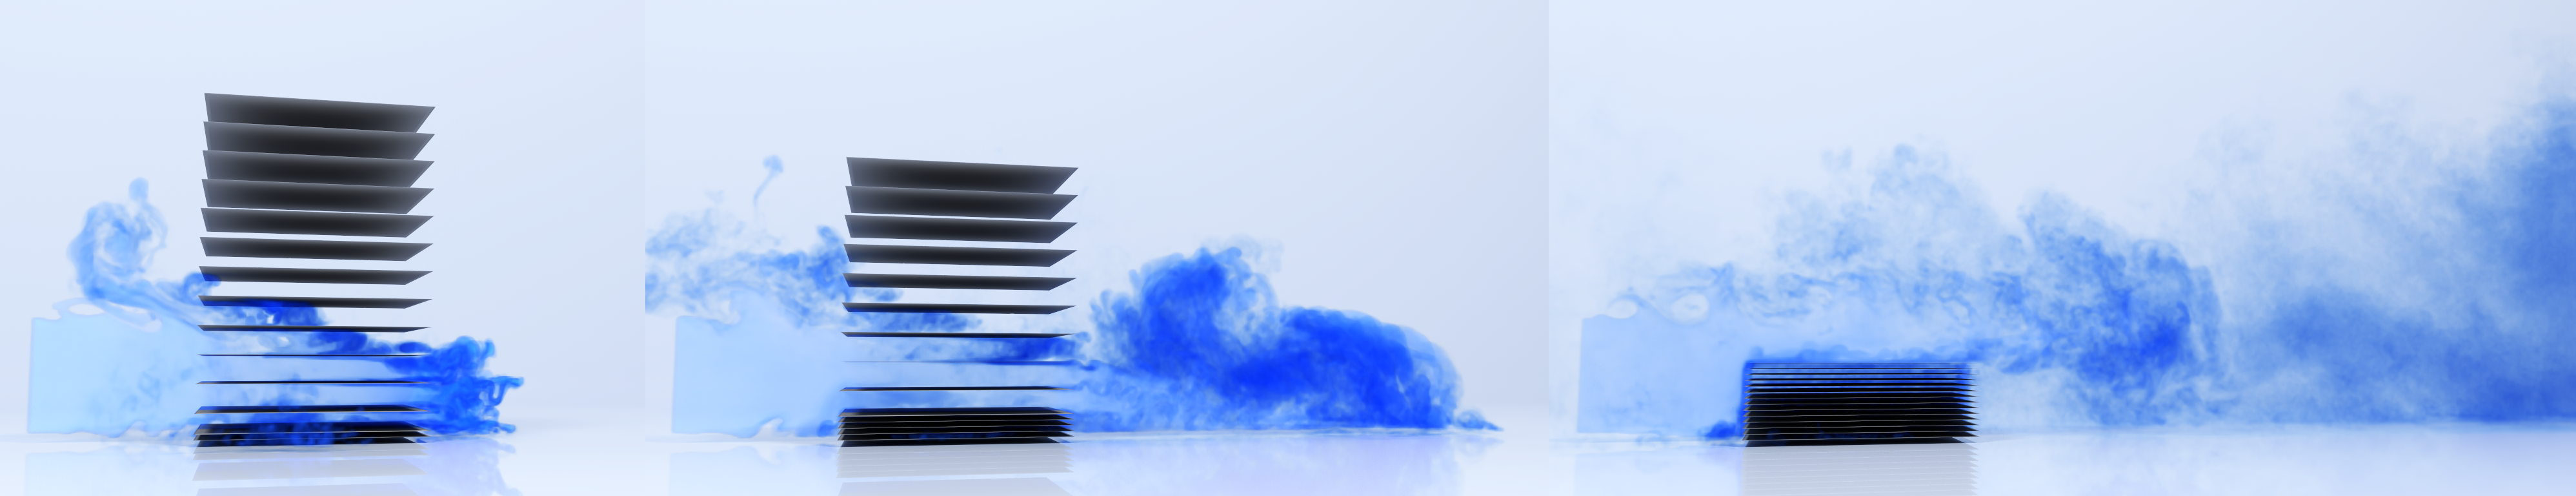
\includegraphics[width=0.99\columnwidth]{figures/result_thin_shell_sub_grid.png}
  \bicaption[烟雾经过层叠的板子]{烟雾经过层叠的板子。烟雾吹过一系列下落的薄板。虽然薄板在分开时烟雾可以通过,当它们层叠在一起时却形成一个密闭的障碍物。我们边界处理中的亚网格近似可以同时处理这两种不同情况,当板子加速靠近时,中间的流体会被加速,而它们紧贴时会成为一个厚的物体。}{Smoke flow through stacked plates. Smoke is blown towards a falling stack of thin plates. While smoke freely flows between separate plates, they become an airtight obstacle when they are stacked on top of each other. Our boundary treatment based on subgrid approximation deals with both cases seamlessly: plates getting closer accelerate the flow in between them, while tightly stacked plates are treated as thick solids.}
  \label{img:result-thin-shell-sub-grid}
\end{figure}

\begin{figure}[!htbp]
  \centering
    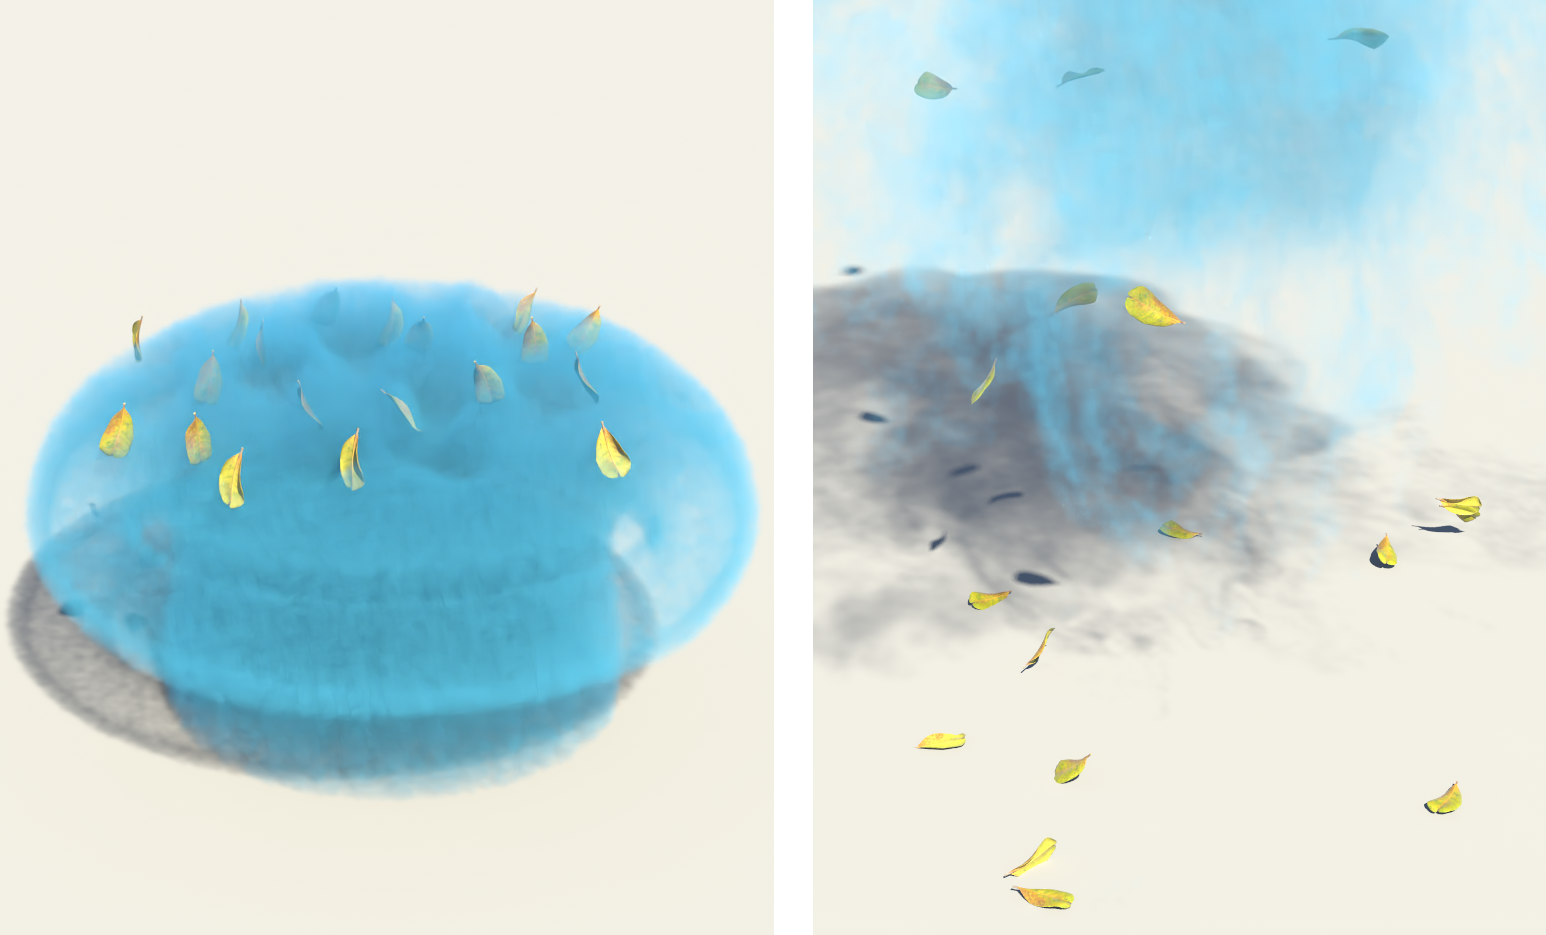
\includegraphics[width=0.99\columnwidth]{figures/result_blowing_leaves.png}
  \bicaption[风吹叶子的仿真]{风吹叶子的仿真。在这个双向流固耦合结果中,一阵风从地面吹起将树叶吹向空中。}{Wind blowing leaves. In this two-way coupling example, a puff of wind from the ground drives a bunch of dried-up leaves up in the air.}
  \label{img:result-blowing-leaves}
\end{figure}

\paragraph{与薄板的耦合}
我们首先构造一个薄圆柱面,使得厚度远小于网格大小,之后令圆柱面旋转,产生剪切流 (见图~\ref{img:result-tube})。我们在低雷诺数 (高黏度) 与高雷诺数 (低黏度) 分别进行了测试,并展示出完全不同的流场特性。我们还测试了多个薄板相叠的场景。这些薄板最初是分开的,之后逐渐叠落在一起。我们的亚网格近似使得我们的方法可以仿真从起初分离的薄板到叠在形成一个固体的整个过程,而无需任何调整。结果可见图~\ref{img:result-thin-shell-sub-grid}。我们最后展示一个双向耦合的结果,仿真一阵风从地面吹起树叶的过程。树叶一开始被风吹起后,缓慢地落回地面,并因风产生旋转。结果可见图~\ref{img:result-blowing-leaves}。

\begin{figure}[!htbp]
  \centering
    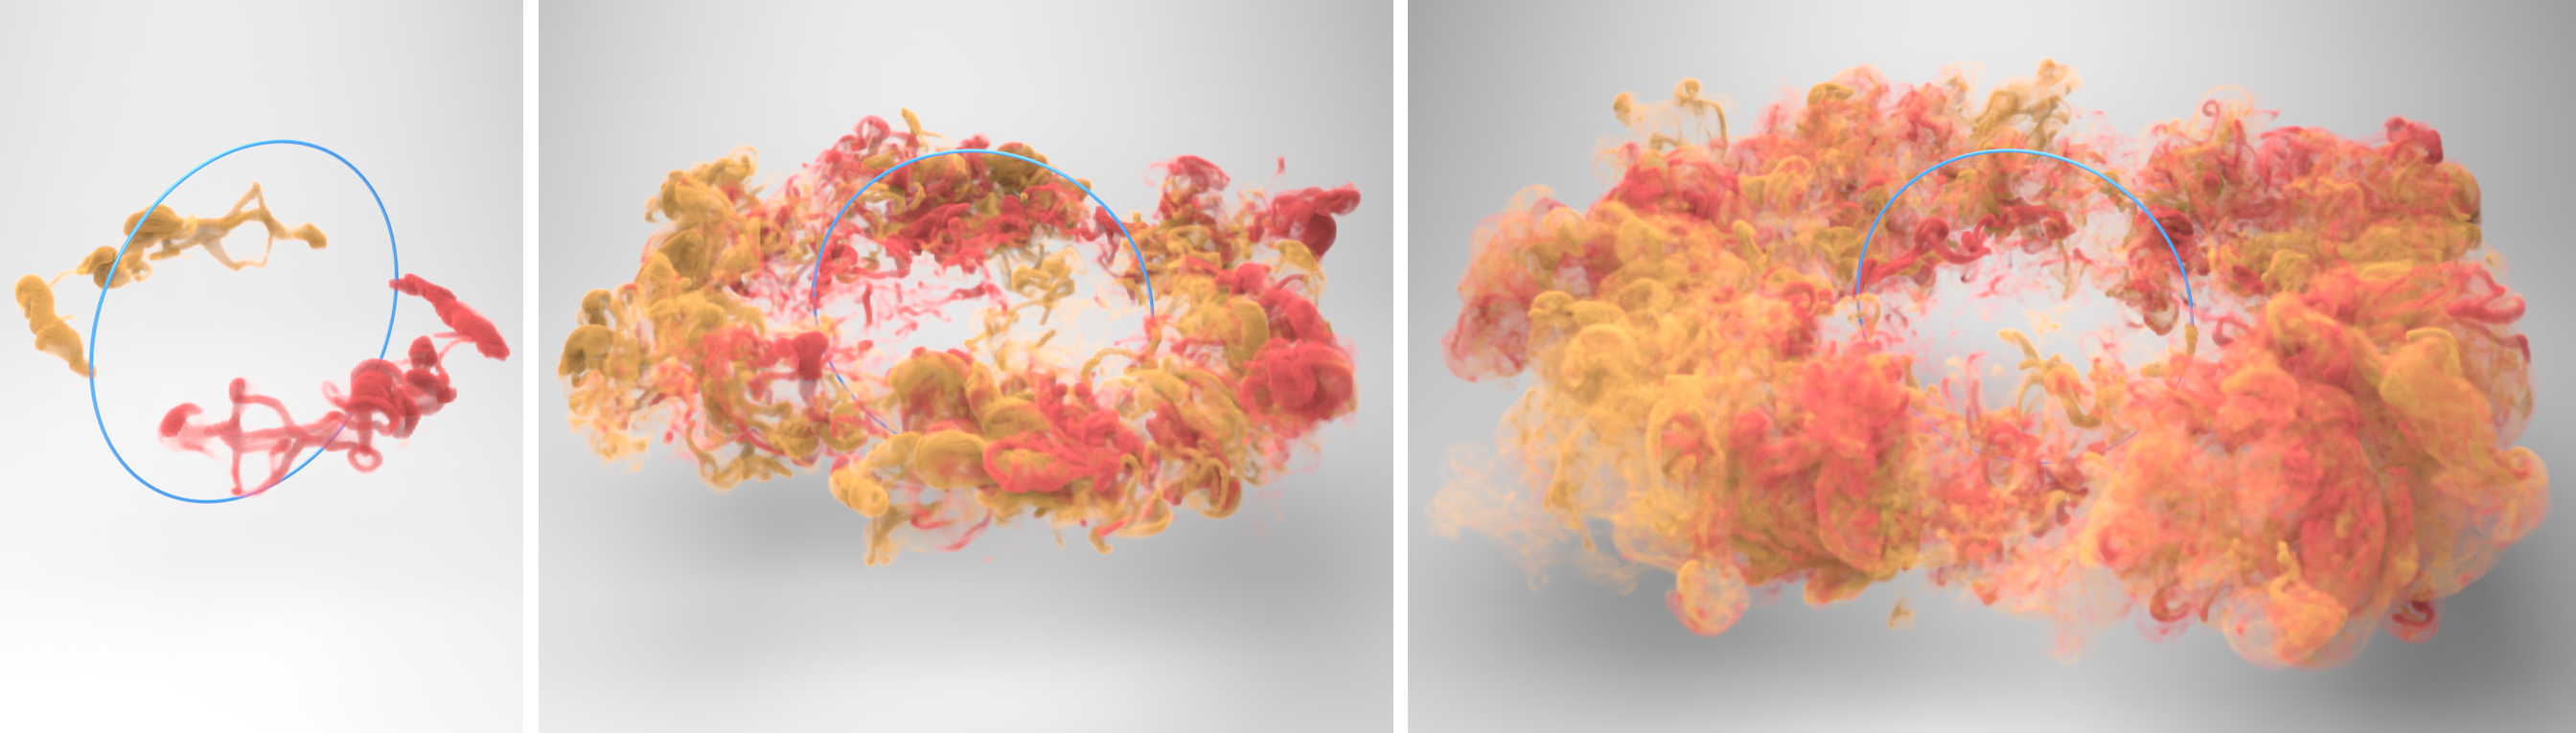
\includegraphics[width=0.99\columnwidth]{figures/result_rotating_torus.png}
  \bicaption[旋转的圆环]{旋转的圆环。一个非常细的圆环沿着一个垂直轴旋转,在两侧发出黄色和橘色的烟雾,展示出圆环旋转所带出的湍流。}{Rotating ring. A very thin ring rotating along a vertical axis and emitting yellow and orange smoke particles is enough to create a turbulent wake as evidenced by the volutes of smoke resulting from the motion.}
  \label{img:result-rotating-torus}
\end{figure}

\begin{figure}[!htbp]
  \centering
    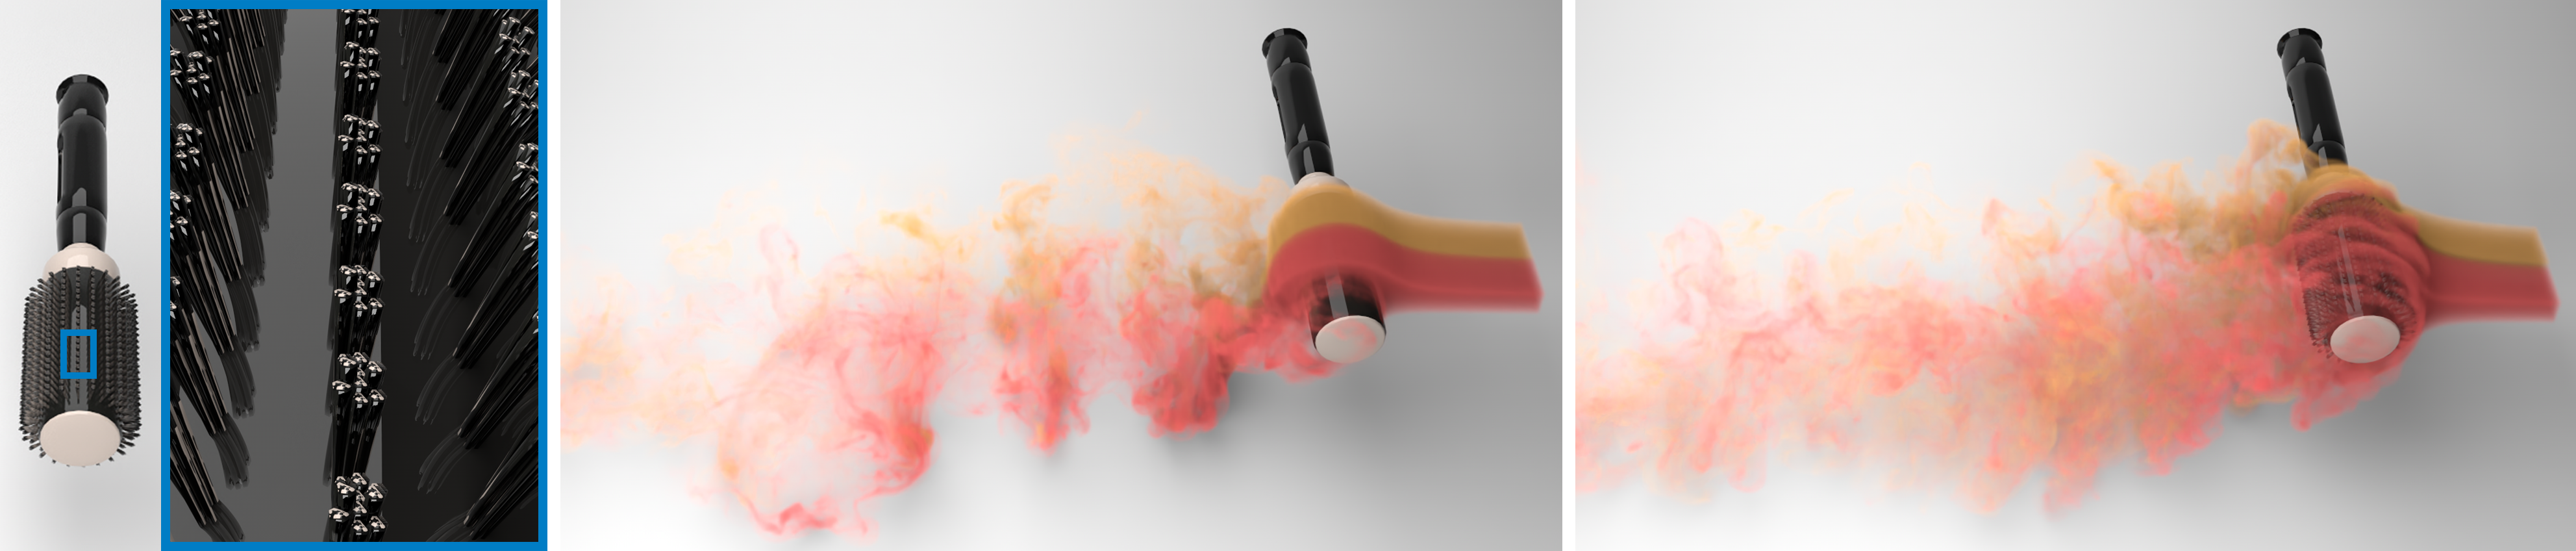
\includegraphics[width=0.99\columnwidth]{figures/result_thin_rod_sub_grid.png}
  \bicaption[发梳仿真]{发梳仿真。一个包含着上百根硬毛的发梳 (左图) 在旋转的同时从左向右平移,带动周围气流运动。与有硬毛的情况 (右图) 相比,没有硬毛时的发梳 (中图) 运动产生的尾流更加平滑,涡旋也更大。这个结果展示了我们的边界处理方法,包括亚网格近似,处理复杂几何的能力。}{Hair brush. The translating and rotating motion of a hair brush containing hundreds of bristles (left) creates fine vortices in its wake as well as around the bristles (right) as evidenced by the evolution of the smoke passing around it, properly capturing the intricate fluid-solid interaction engendered by this complex geometry. Compared to the coupling with bristles (right), the smoke near the hair brush without bristles (middle) is much smoother, and the wake flows contain relatively large vortices, indicating the efficacy of subgrid approximation in handling such complex solid shapes.}
  \label{img:result-thin-rod-sub-grid}
\end{figure}

\paragraph{与细棒的耦合}
下面继续展示我们的求解器对细棒耦合的仿真结果。我们先展示一个环状物体在空气中定速旋转的结果,其直径远小于网格大小,见图~\ref{img:result-rotating-torus}。我们还对多个细棒组合在一起时的情况进行仿真,结果见图~\ref{img:result-thin-rod-sub-grid}。注意当固体表面有硬毛时,尾流的湍流程度有显著的差别。

\begin{figure}[!htbp]
  \centering
    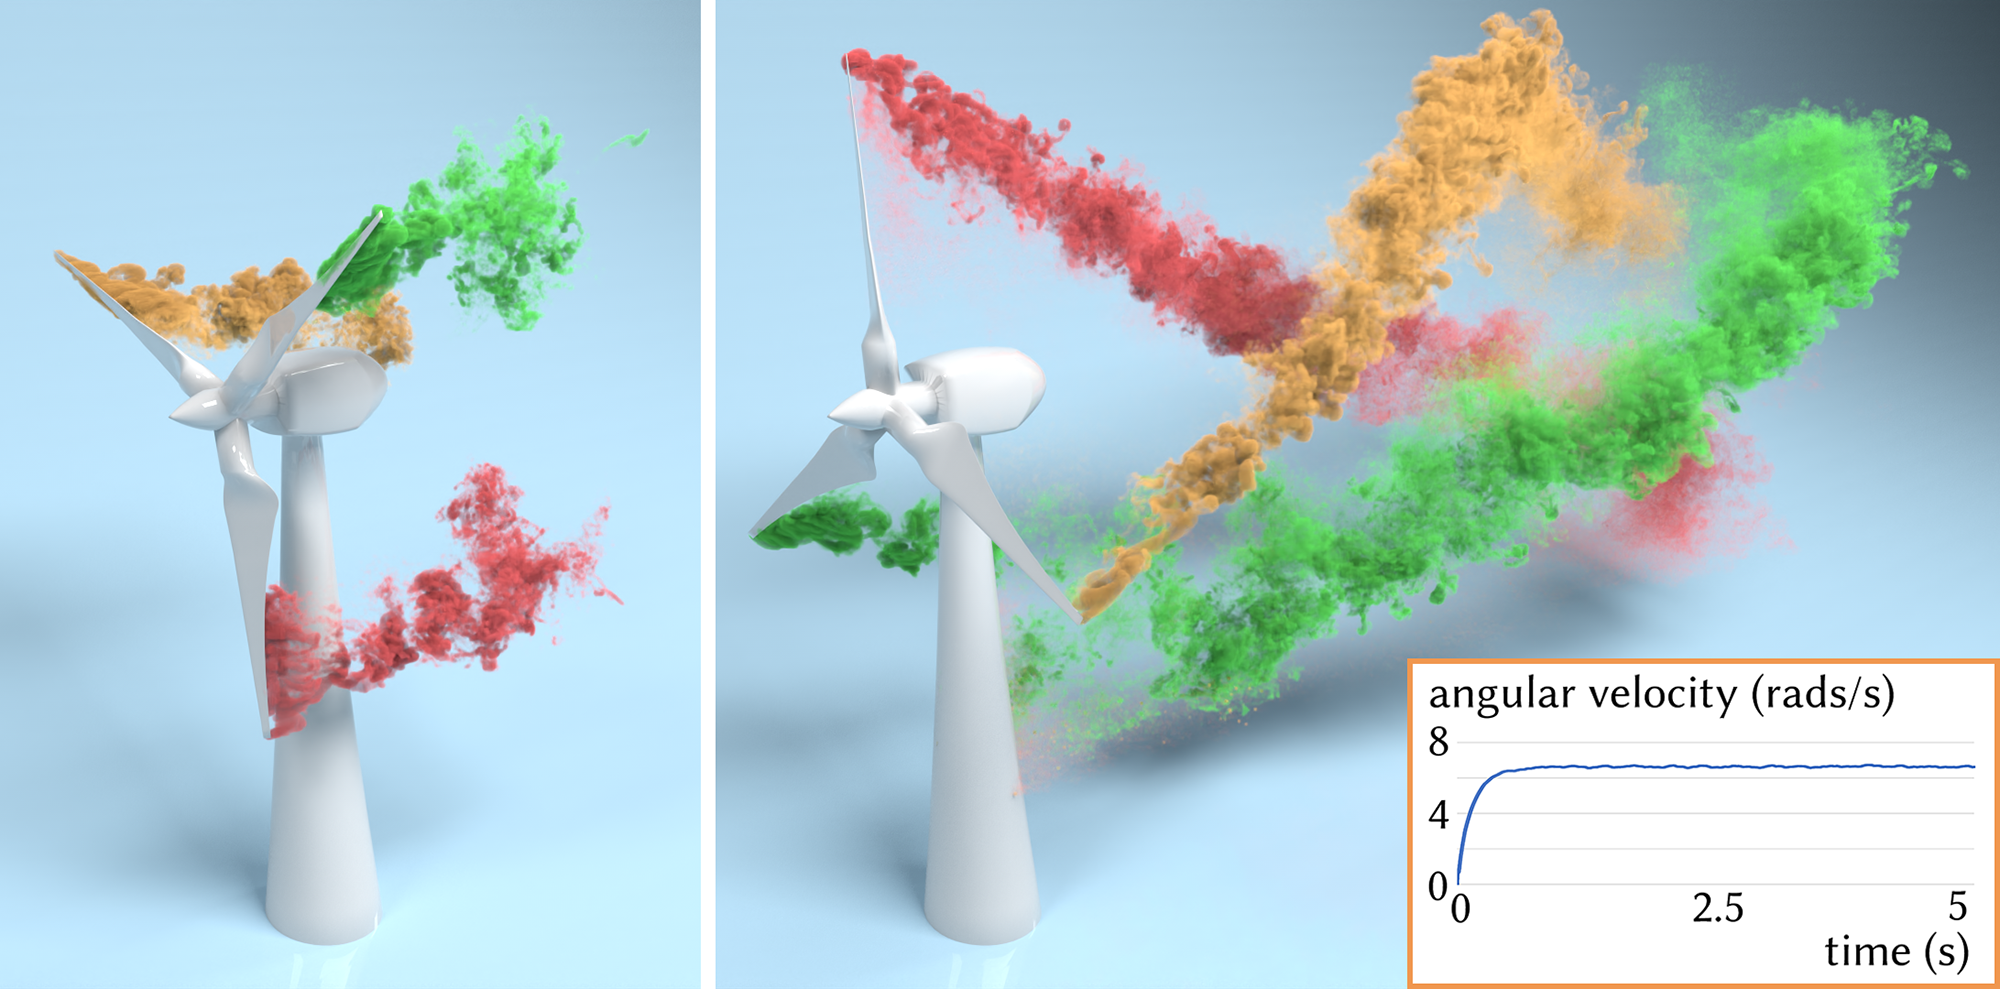
\includegraphics[width=0.99\columnwidth]{figures/result_wind_turbine.png}
  \bicaption[风力涡轮机的仿真]{风力涡轮机的仿真。常速的风吹过一个有三个扇叶的风力涡轮机,驱动涡轮机旋转,并由扇叶上产生的烟雾对涡旋尾流结构进行可视化。这个双向的流固耦合结果考虑了轴上的摩擦力来限制了最大的角速度。扇叶角速度随时间的变化可见底部的小图。}{Turbine. A large turbine emitting colored smoke particles at the three propellers of its large blade is simulated with a constant incoming air flow making it turn, creating a spiral vortex trail. This two-way coupling example also involves friction on the axis of the turbine to limit its maximum angular velocity, resulting in a time-varying but converging curve of angular velocity of the turbine shown in the bottom inset.}
  \label{img:result-wind-turbine}
\end{figure}

\begin{figure}[!htbp]
  \centering
    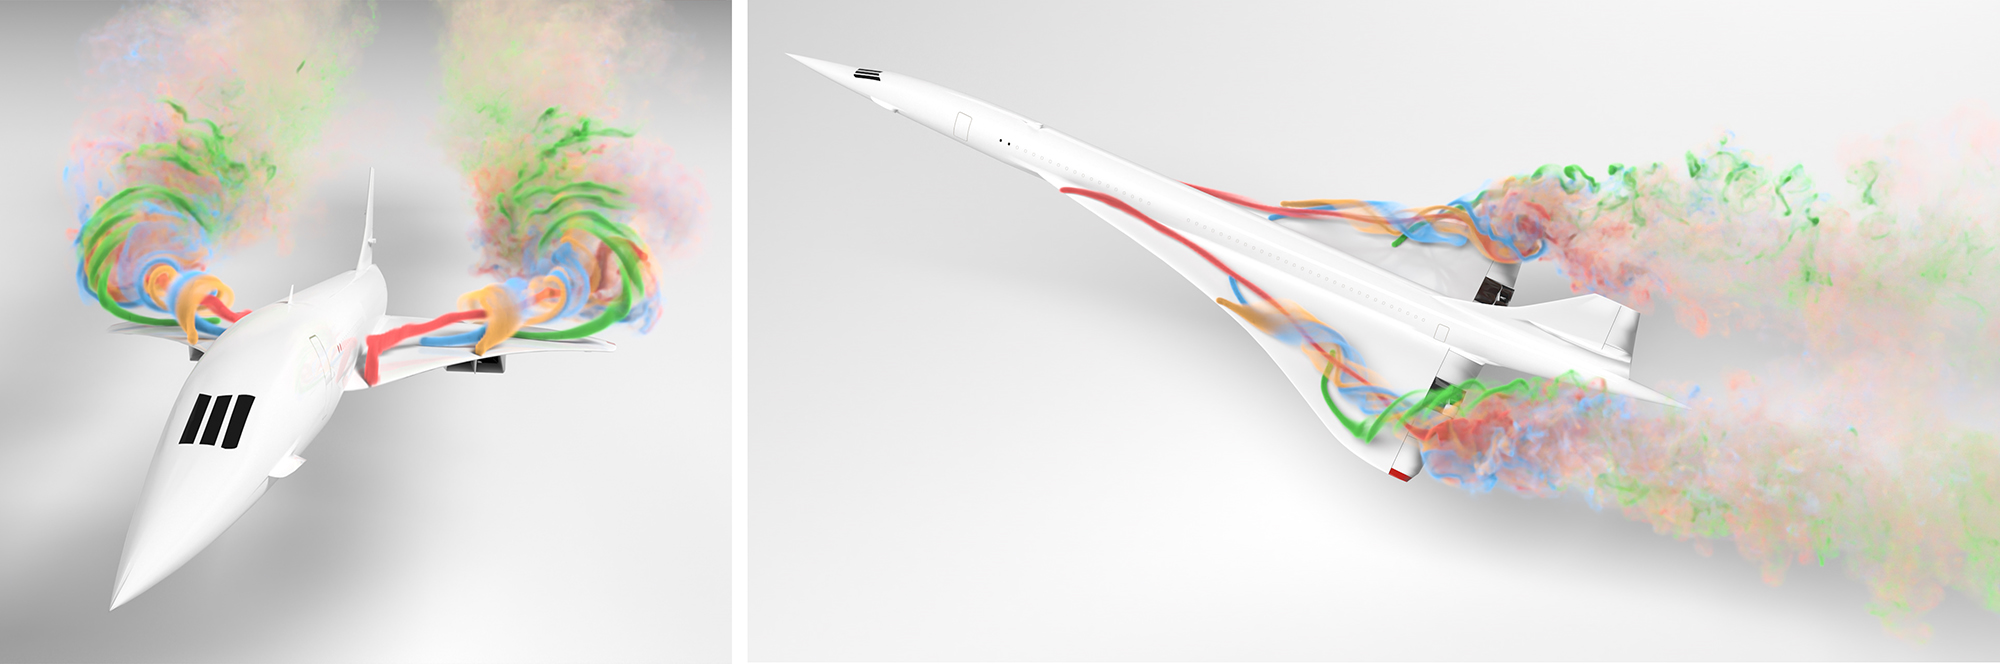
\includegraphics[width=0.99\columnwidth]{figures/teaser_concorde.jpg}
  \bicaption[飞机气动仿真]{飞机气动仿真。通过对协和客机翼面的气流仿真,我们展示出我们的方法可以同时处理含有薄板、细棒的薄物体以及厚物体的复杂几何。}{Aerodynamic simulation of an airplane. By simulting the flow over the wing of the Concorde airplane, we demonstrate that our method can handle complex solids containing thin shells, rods and thick objects.}
  \label{img:teaser_concorde}
\end{figure}

\paragraph{与复杂物体耦合}
一个更复杂但非常常见的情况是厚物体与薄物体同时存在,并共同构成一个复杂物体。我们的边界处理可以有效并统一地处理这种情况。图~\ref{img:result-wind-turbine} 展示了通过风带动一个三扇叶风力涡轮机模型旋转的仿真结果。这里风在带动扇叶旋转的同时,扇叶也影响空气流动,展现了我们方法处理复杂物体的双向耦合。图~\ref{img:teaser_concorde} 展示了协和式客机以攻角20度姿态在空中飞行的仿真结果。对于飞机这样的复杂物体,许多部件对于网格都是亚网格大小的,尤其是机翼部分。在这两次仿真中,得到的结果都与期望相符。

\begin{figure}[!htbp]
  \centering
    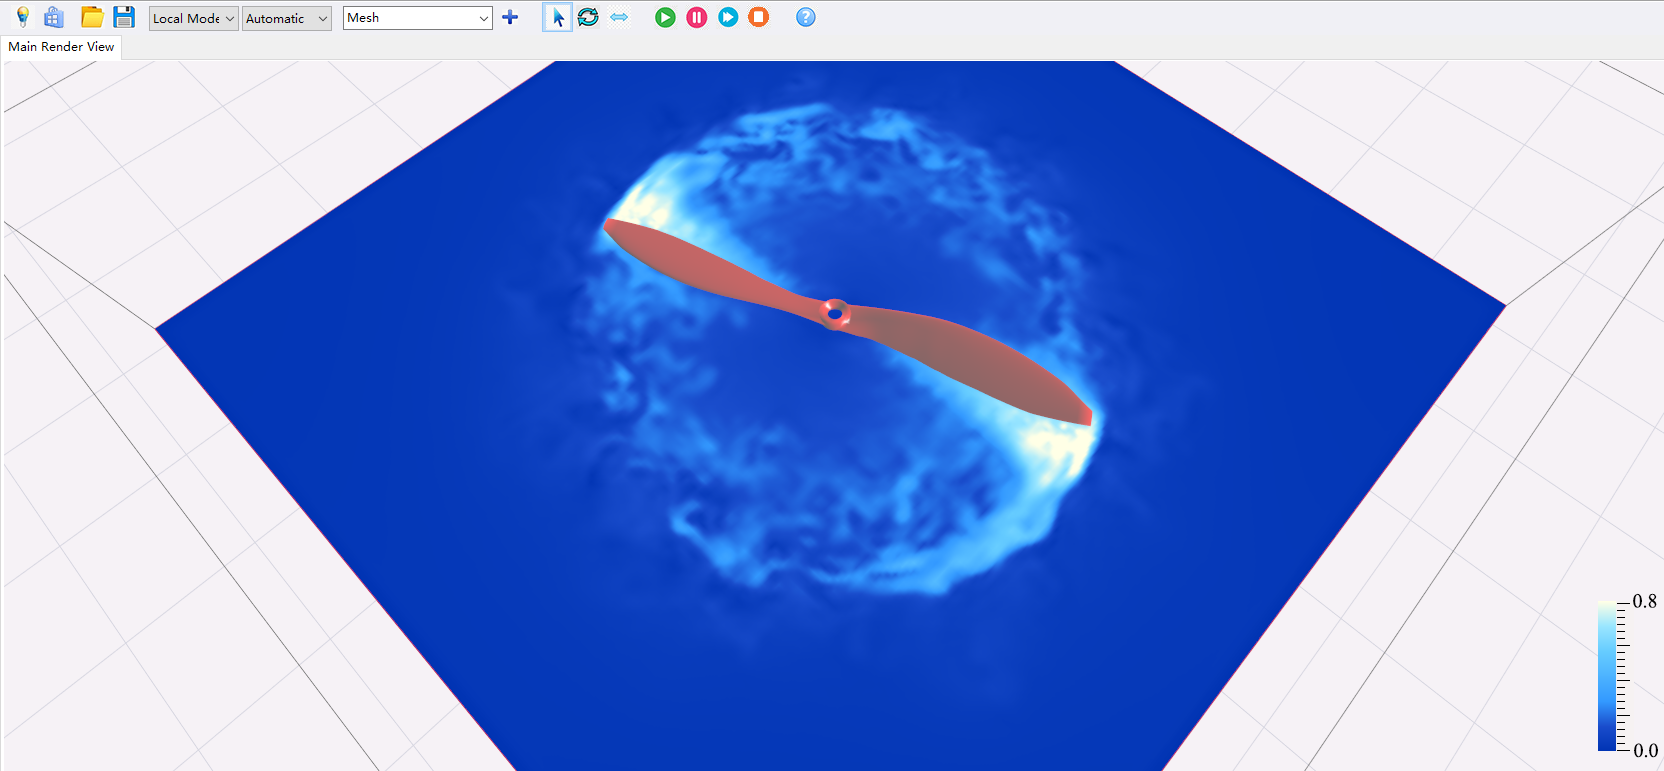
\includegraphics[width=0.99\columnwidth]{figures/result_design.png}
  \bicaption[快速交互设计]{快速交互设计。我们通过GUI操作模拟系统,来快速生成仿真结果。图中示例为一个快速旋转的旋翼,我们可以通过可视化即时的看到尾流情况。这样的快速交互式仿真可以用来辅助产品设计与验证。}{Fast simulation for interactive design. We operated our GUI-based simulation system to produce a quick preliminary result of a fast rotating rotor-blade where turbulent wake flows can be observed interactively, which is very useful for efficient product design and verification.}
  \label{img:result-design}
\end{figure}

\begin{figure}[!htbp]
  \centering
    \includegraphics[width=0.99\columnwidth]{figures/result_city.png}
  \bicaption[气流经过城市街区的高分辨率仿真]{气流经过城市街区的高分辨率仿真。我们对气流经过城市街区进行高分辨率仿真 (($889\times333\times556$)),建筑中包含诸多细且尖锐的结构。一层相对薄的烟雾从左侧注入,在建筑间产生涡流细节。}{High-resolution simulation of airflow through a city neighborhood. We simulate the airflow passing around and over buildings using a high resolution grid ($889\times333\times556$), where the buildings contain both thin and sharp structures. A layer of smoke particles with relatively small thickness is coming from the left, creating fine vortical structures behind and in between the buildings.}
  \label{img:result-city}
\end{figure}

\begin{figure}[!htbp]
  \centering
    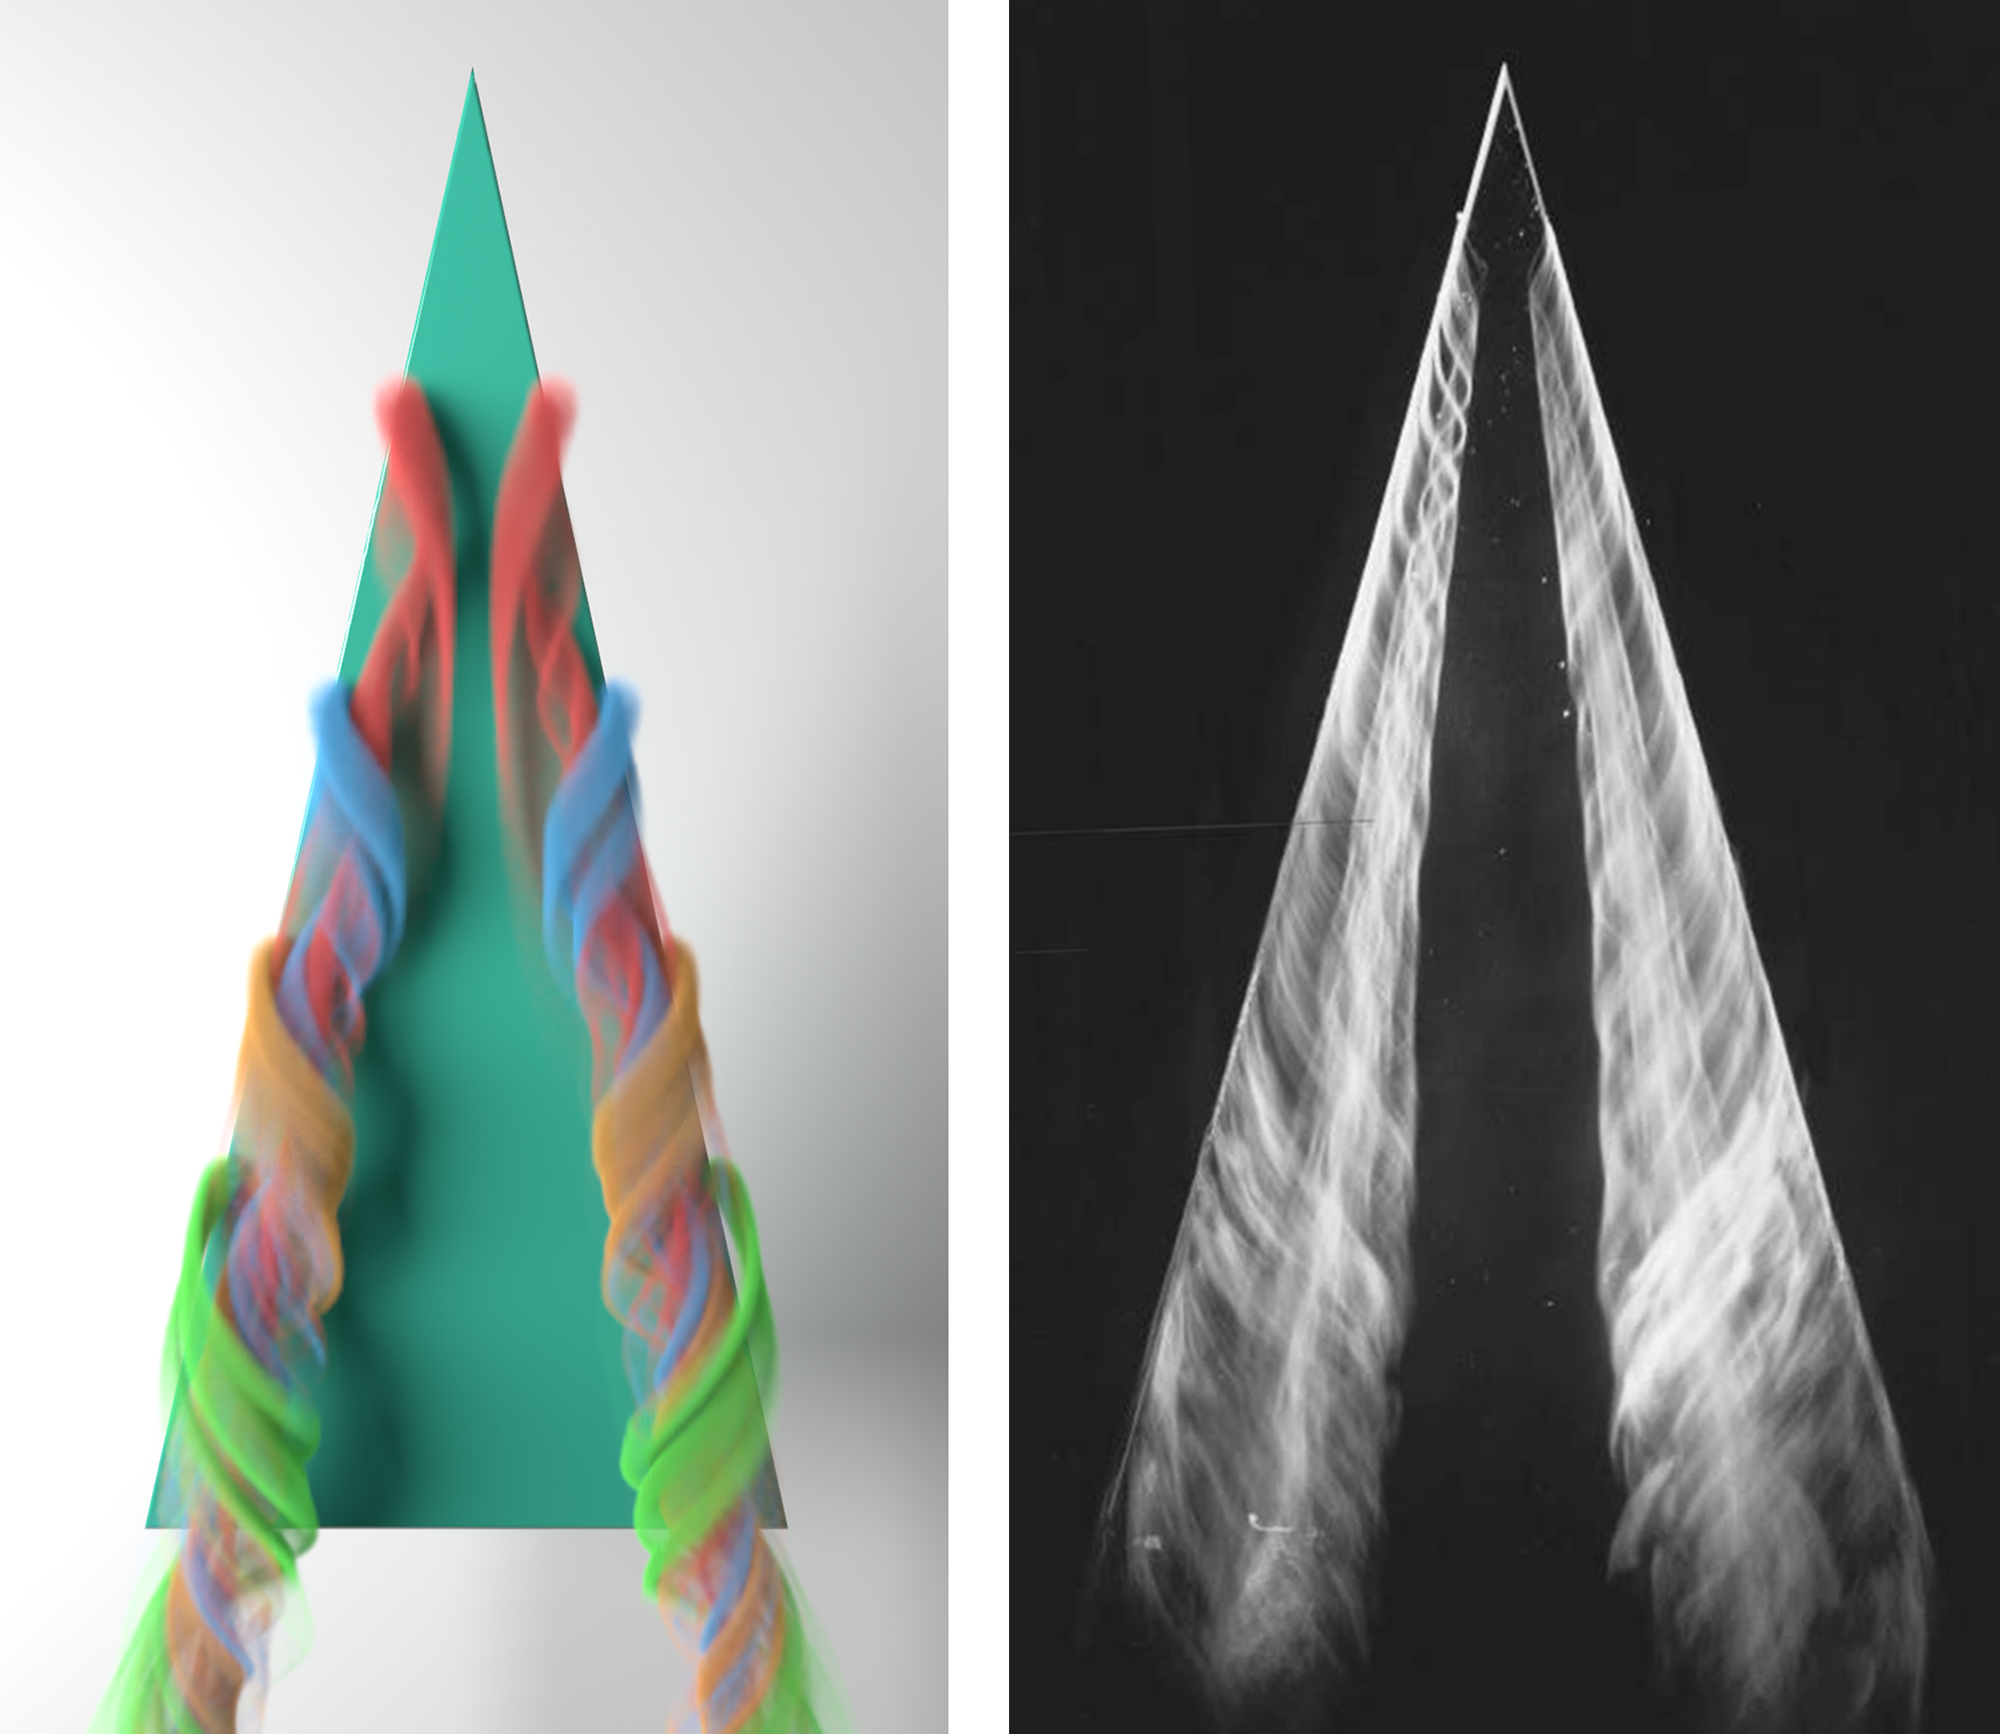
\includegraphics[width=0.99\columnwidth]{figures/comparison_delta_wing.png}
  \bicaption[三角翼仿真]{三角翼仿真。通过我们的图形方法得到的薄板三角翼仿真结果 (左图) 与实际实验~\cite{Delery:2001} (右图) 的对比,展示出相同的前缘涡旋结构,表面我们的图形方法在薄结构边界层上的准确性。}{Delta-wing simulation. The airflow over a thin-shell delta-wing simulated with our hybrid coupling approach (left) matches experimental visualizations from~\cite{Delery:2001} (right), exhibiting the same spiral vortex structure near the leading edge of the wing and demonstrating the accuracy of our solver in capturing boundary layer flows around thin structures.}
  \label{img:comparison_delta_wing}
\end{figure}

\begin{figure}[!htbp]
  \centering
    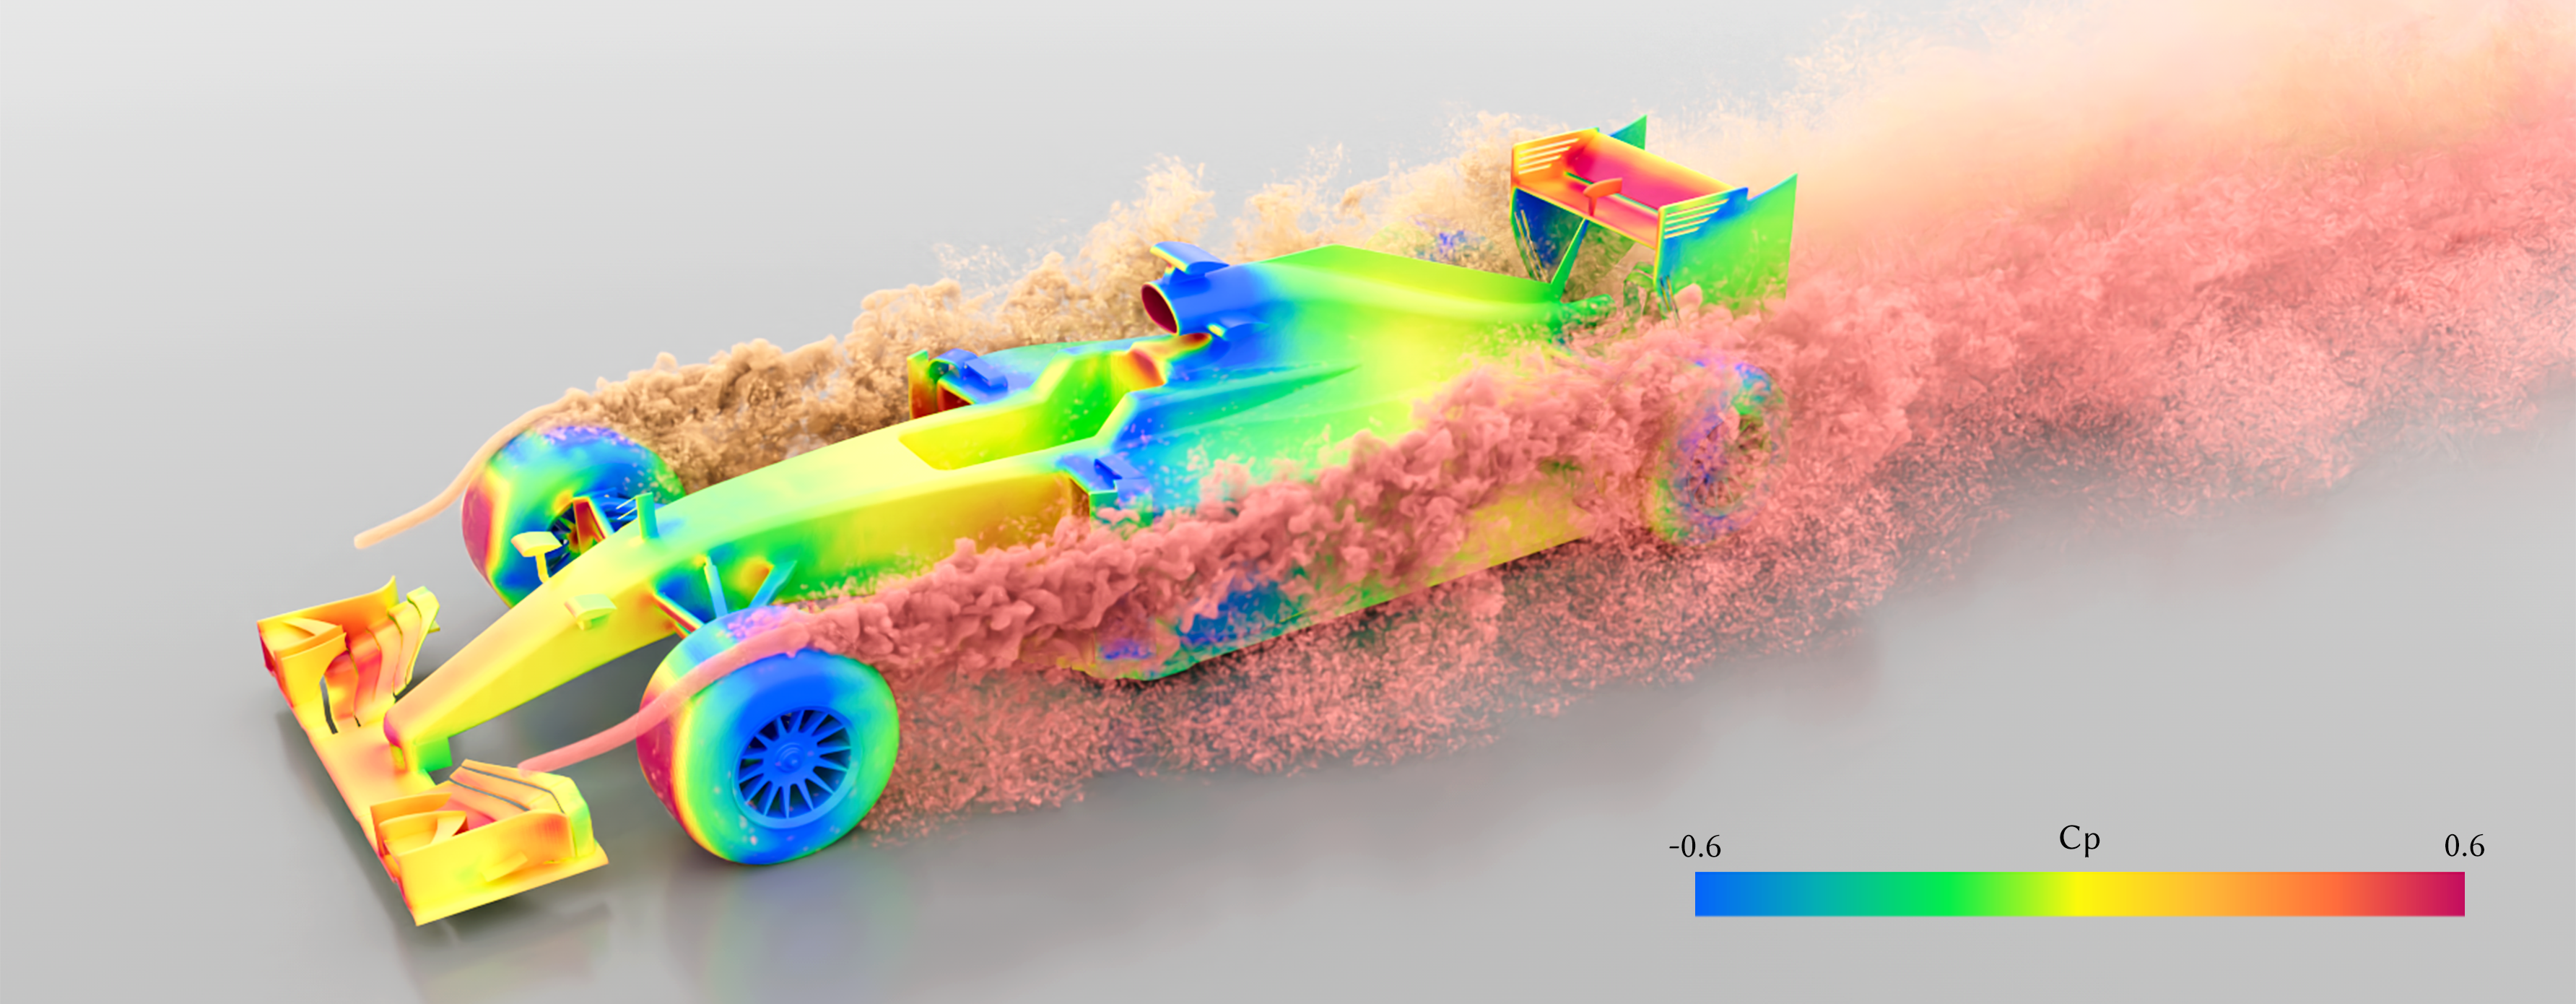
\includegraphics[width=0.99\columnwidth]{figures/teaser_f1.png}
  \bicaption[F1赛车的气动仿真]{F1赛车的气动仿真。这里,车身表面上显示了平均压力场 ($C_\text{p}$),车前的两个发射源中发出染色的粒子对车身及转动的轮胎后方的尾流进行可视化。该仿真使用了五层网格,最细的网格大小为4mm,F1赛车的车身为4.15m。通过我们的GPU加速实现,我们完成了2秒的仿真,在精度可用于工业仿真的同时,仿真耗费的计算时间不足1个小时。}{Aerodynamics of an F1 racing car. Here, the mean pressure field ($C_\text{p}$) is shown on the car body surface, while passively-advected dyed particles from two front sources show the wake flow behind the rotating wheels and the car body. Five-level multiresolution grids are used to capture an effective resolution of 4mm on the body of an F1 racing car measuring 4.15 meters. 
  With our optimized GPU implementation, a 2-second simulation of such a complex model takes less than one hour to compute, with an accuracy meeting current industrial standards for automotive aerodynamics. }
  \label{img:teaser_f1}
\end{figure}

\begin{figure}[!htbp]
\centering
  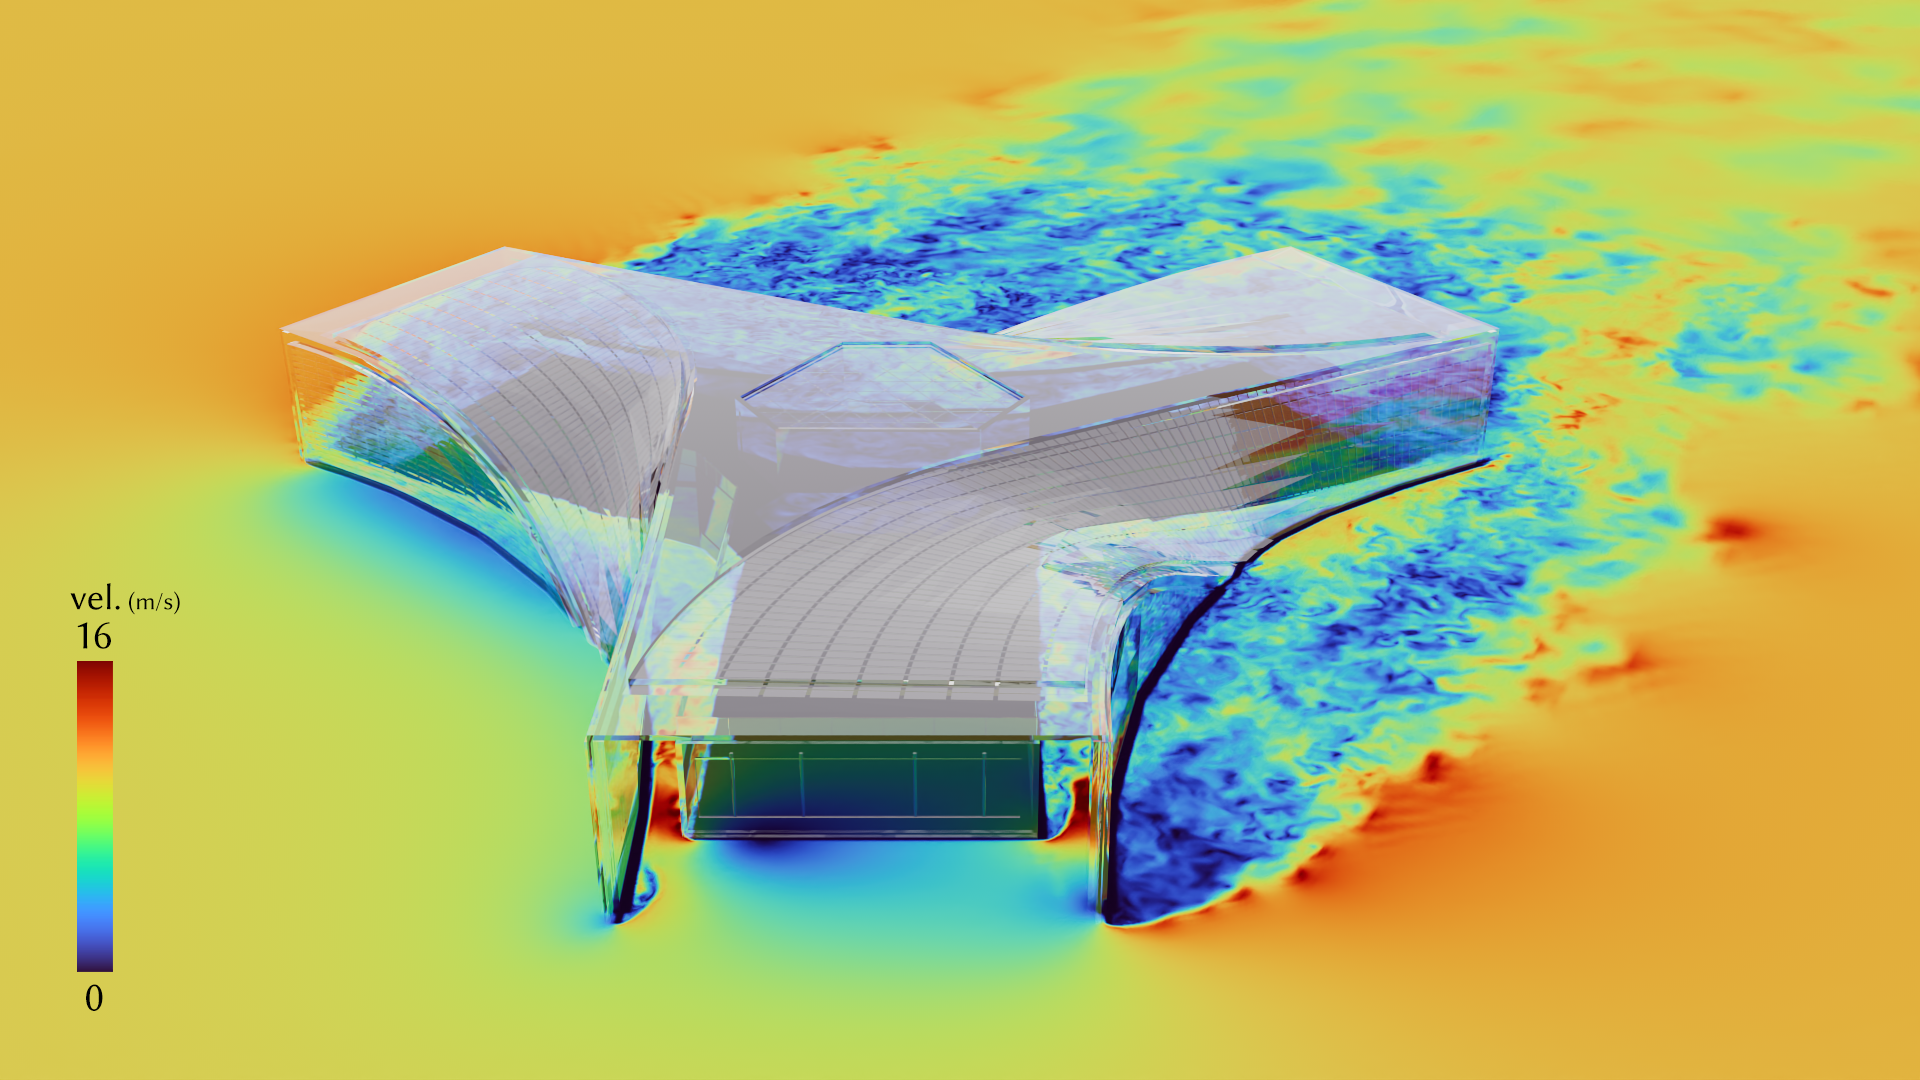
\includegraphics[width=0.99\columnwidth]{figures/vis_building.png}
\bicaption[建筑模型的气动仿真]{建筑模型的气动仿真。我们的虚拟风洞系统可以对包含多个通道在内的建筑结构进行仿真。从结果中我们可以清晰地看到模型内部的流场。图中通过颜色可视化的水平截面为速度场模值。}{Aerodynamics of an architectural model. Our virtual wind tunnel can simulate the airflow passing through a building structure containing covered passages inside. Visualized here is the velocity field magnitude for a horizontal cross-section, where the internal flow is clearly visible.}
\label{img:vis_building}
\end{figure}

\begin{figure}[!htbp]
\centering
  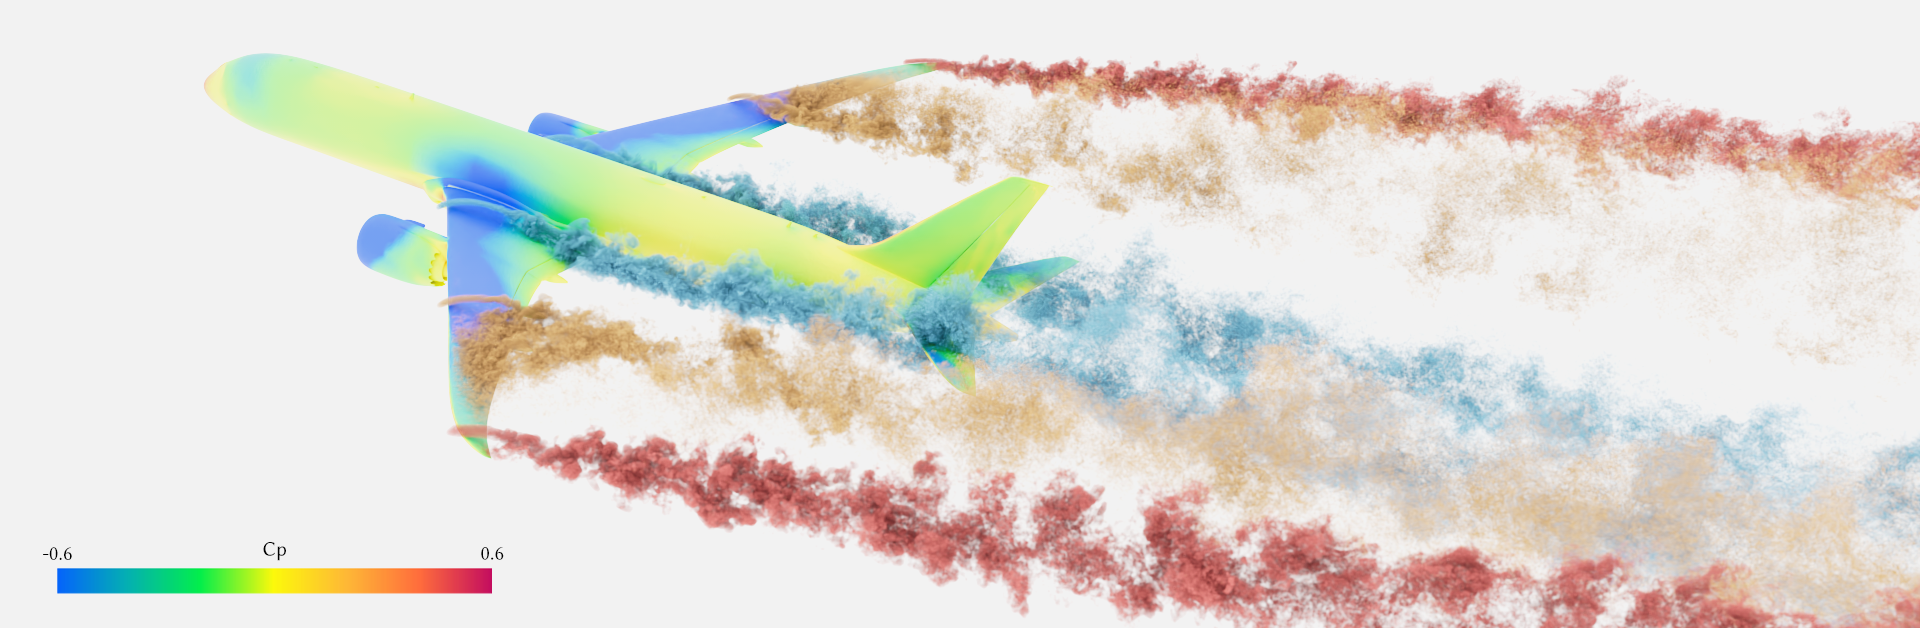
\includegraphics[width=0.99\columnwidth]{figures/vis_plane.png}
\bicaption[波音787客机的气动仿真]{波音787客机的气动仿真。我们在两个GPU上对缩比的波音787客机模型进行了高分辨率仿真,客机的攻角为$8^{\circ}$。客机表面通过颜色对表面压力场进行了可视化,并有从6个沿着机翼前缘不同位置发出的染色粒子对流体进行被动追踪。}{Aerodynamics of a Boeing-787 passenger aircraft. We conducted a high-resolution aerodynamic simulation on dual GPUs for a scaled aircraft model of Being 787 at an angle of attack of $8^{\circ}.$
The pressure field is color-mapped over the aircraft body surface, while passively-advected dyed particles injected from the six different locations along the leading edge of the main wing are visualized.}
\label{img:vis_plane}
\end{figure}

\begin{figure}[!htbp]
\centering
  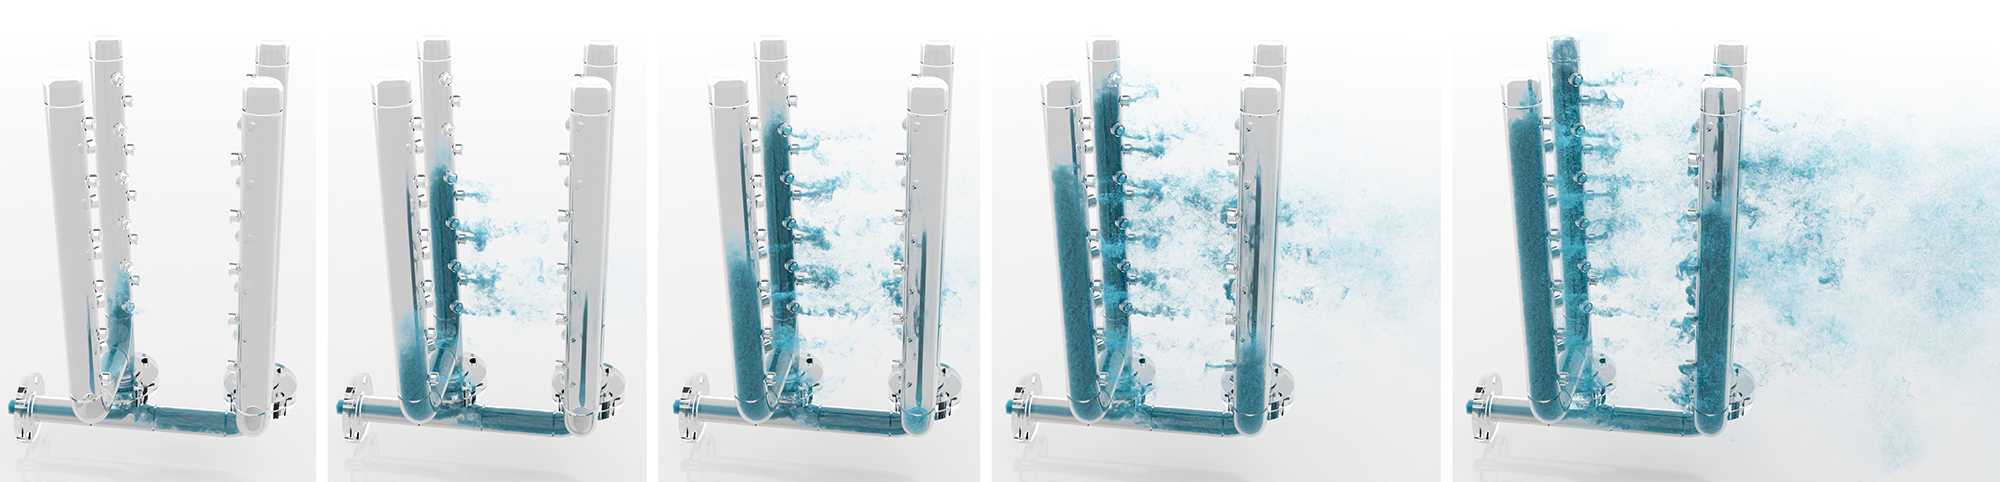
\includegraphics[width=0.99\columnwidth]{figures/vis_pipe.png}
\bicaption[气流经由一个有喷嘴的管道流出]{气流经由一个有喷嘴的管道流出。我们使用我们的方法,基于多分辨率网格,可以仿真气流流过一个有很多喷嘴的管道。管道表面被渲染为半透明以看清楚其中的流场。烟雾粒子从管道的入口喷入,并逐渐充满管道后,从喷嘴中流出。注意管道周围的空气是以定速向右流动的,所以烟雾粒子从喷嘴中喷出后会继续向右流动。}{Airflow passing through a pipe with nozzles. With our multiresolution solver, we can simulate a flow passing through an irregular transparent pipe with various nozzles on its surface. By injecting smoke particles at the inlet of the pipe, it becomes clear that the flow gradually fills up the pipe while exiting from the nozzles. Note that the surrouding air was given an initial constant velocity, which blows the smoke rightward after it comes out.}
\label{img:vis_pipe}
\end{figure}

\paragraph{快速仿真以进行交互式设计}
我们的流固耦合算法可足够高效,以进行交互式产品设计与测试。作为示例,我们在$200\!\times\!200\!\times\!200$分辨率下对一个旋翼旋转的情况进行仿真。图~\ref{img:result-design} 展示了仿真中的速度场截面。完成1/100秒的仿真所需的计算时间约为0.4秒。这个时间包括数据的读取与可视化 (截面可视化在CPU上完成)。这意味着类似旋翼这类的产品可以使用我们的算法进行快速的气动性能评估,并可基于此优化设计。

\paragraph{大规模仿真}
最后,我们展示一个相对高分辨率的大规模仿真结果,来展示我们方法的可扩展性。该仿真使用两个GPU同时计算,展示了大量烟雾穿过一个高密度城市街区的场景 (见图~\ref{img:result-city})。场景中包含诸多细且尖锐的物体对尾流产生影响。对于这样的大场景湍流仿真,5秒的仿真所需的计算时间为1.5小时左右。正如Li等~(\citeyear{Li-2020}) 所讨论的,达到这样的仿真效率对于N-S方法来说是十分困难的,即使同样使用多GPU进行加速。主要原是N-S方法中压力场求解这一步需要求解全局的线性方程组,在高分辨率下会严重影响计算效率。

\paragraph{实际物理现象的定性复现}
为了进一步验证我们方法在有亚网格物体时边界处理的精度,我们与现实世界中的实验进行定性地复现。
首先我们对三角翼的风洞实验进行复现。该三角翼的后掠角度为$75^\circ$,攻角为$20^\circ$ (见图~\ref{img:comparison_delta_wing} (a))。在实验中,三角翼上方会产生稳定的螺旋涡流结构,提升气动升力 (这种升力被称为涡升力~\cite{anderson2010aircraft})。这种结构被广泛使用于现代飞行器的设计中,如图~\ref{img:teaser_concorde} 中的协和客机。该实验的可视化可见图~\ref{img:comparison_delta_wing} (b)~\cite{Delery:2001}。我们的仿真结果在视觉上与实验结果相匹配,展示出相似的螺旋涡流结构。

虽然在第~\ref{sec:sig23} 章中,我们主要讨论了如何将该方法应用至工业计算领域,但我们也有一个重要的动机是通过提出一个高精度的流体仿真方法,弥合CG与CFD领域中计算方法的差异。为了展示该方法不止有能力应用于工业领域的仿真,也可以在视觉特效领域,仿真极为复杂的流体现象,以用于真实的视觉特效制作。我们接下来展示一系列使用第~\ref{sec:sig23} 章中的方法得到的面向视觉动画的仿真结果。

图~\ref{img:vis_plane}、\ref{img:teaser_f1} 与~\ref{img:vis_building} (包括下一节中的图~\ref{img:golf_ball_vis}、\ref{img:golf_ball_comp_single_res}、\ref{img:fastback}) 中都包含速度场截面的可视化,这里的可视化是将速度场的模值映射到了不同的颜色上。在映射时,整个网格的速度场通过格点上的速度线性插值获得。我们同时也在一些结果中展示了物体表面的压力系数$C_\text{p}$。为了获得物体表面的压力系数,我们需要将最贴近物体表面的压力场投影至物体表面。但是注意到因为切削网格造成的影响,不同切削网格点距物体表面的距离是不同的。如果我们只将距离物体表面最近的格点的压力投影至物体表面,它们的压力是不连续的。为了解决这一问题,我们从物体表面出发,沿法向方向走固定距离 (通常为一个网格大小),然后在该处通过插值获得压力值后,再投影至物体表面。这样我们可以获得更连续的物体表面压力可视化,如图~\ref{img:teaser_f1}。

根据模型的尺度、计算域的大小与最细网格大小的不同,整个仿真计算过程可能需要几个小时。其中我们的多分辨率网格构建过程一般需要不多于20分钟。

\paragraph{飞机模型仿真}
首先,我们对一个缩比的波音787飞机模型进行了高分辨率仿真 (见图~\ref{img:vis_plane})。该场景中,飞机的速度相对较低 (0.16马赫),攻角为8度。飞机的长度为6.16米,翼展为3.2米。该仿真在两个NVIDIA A100 GPU上完成,最细的网格分辨率为3.75毫米。完成1.7秒仿真消耗的计算时间约为1.8小时。

\paragraph{F1赛车仿真}
我们还对一个F1赛车模型进行了仿真,以展示我们的动态耦合 (见图~\ref{img:teaser_f1})。仿真过程中,轮胎在不停旋转,对赛车尾部的湍流产生影响。F1赛车的车身为4.15m,仿真时使用的计算域大小为$15m\!\times\!4m\!\times\!6m$,完成2秒仿真消耗的计算时间约为0.9小时。

\paragraph{建筑模型仿真}
我们之后对一个复杂的缩比建筑模型进行了气流仿真。这个模型中包含了一些连通的通道,需要我们通过传播算法来识别所有有效的流体点 (见图~\ref{img:grid_construction})。
该模型的包围盒大小为$4.34m\!\times\!1.06m\!\times\!3.76m$,仿真时使用的计算域大小为$25m\!\times\!8m\!\times\!25m$。完成3.5秒仿真消耗的计算时间约为1.9小时,速度场截面的可视化结果可见图~\ref{img:vis_building}。

\paragraph{管道流仿真}
为了进一步说明我们的方法求解复杂模型边界与拓扑的能力,我们对一个不规则的有喷嘴的管道进行气流仿真 (见图~\ref{img:vis_pipe})。其中,喷嘴将管道的内部与外界连通。
管道模型的包围盒大小为$1.3m\!\times\!2m\!\times\!0.83m$,仿真时使用的计算域大小为$7.84m\!\times\!12m\!\times\!4.96m$。完成6秒仿真消耗的计算时间约为0.9小时。
通过染色的烟雾粒子进行可视化,我们可以很清楚地看到气流通过左下的入口流入管道,并从喷嘴中流出。这展示了我们的方法可以很好地对复杂形状的几何完成自动网格构建。

\section{面向工业应用的仿真结果与对比}
我们现在讨论对本文第~\ref{sec:sig23} 章中所描述的虚拟风洞系统进行的面向工业应用的测试,以验证我们方法的精度与效率。
在仿真中,物体的放置位置根据场景需求而定。对于需要在空中的物体,一般我们放置在竖直方向的中间位置。在地面上的物体则会根据需求设置离地的距离 (如汽车轮胎有时需要陷入地面以弥补轮胎自身的弹性对仿真的影响)。在水平面上,一般物体都会被放置在距来流3分之1的位置 (沿来流方向)。在垂直于来流的方向上,一般物体被放在计算域中间以更好地捕捉尾流。
整个计算域的大小一般是模型包围盒的8到10倍,图~\ref{img:domain_setup} 展示了汽车仿真的计算域场景设置。

\label{sec:results_industry}
\begin{figure}[!htbp]
  \centering
    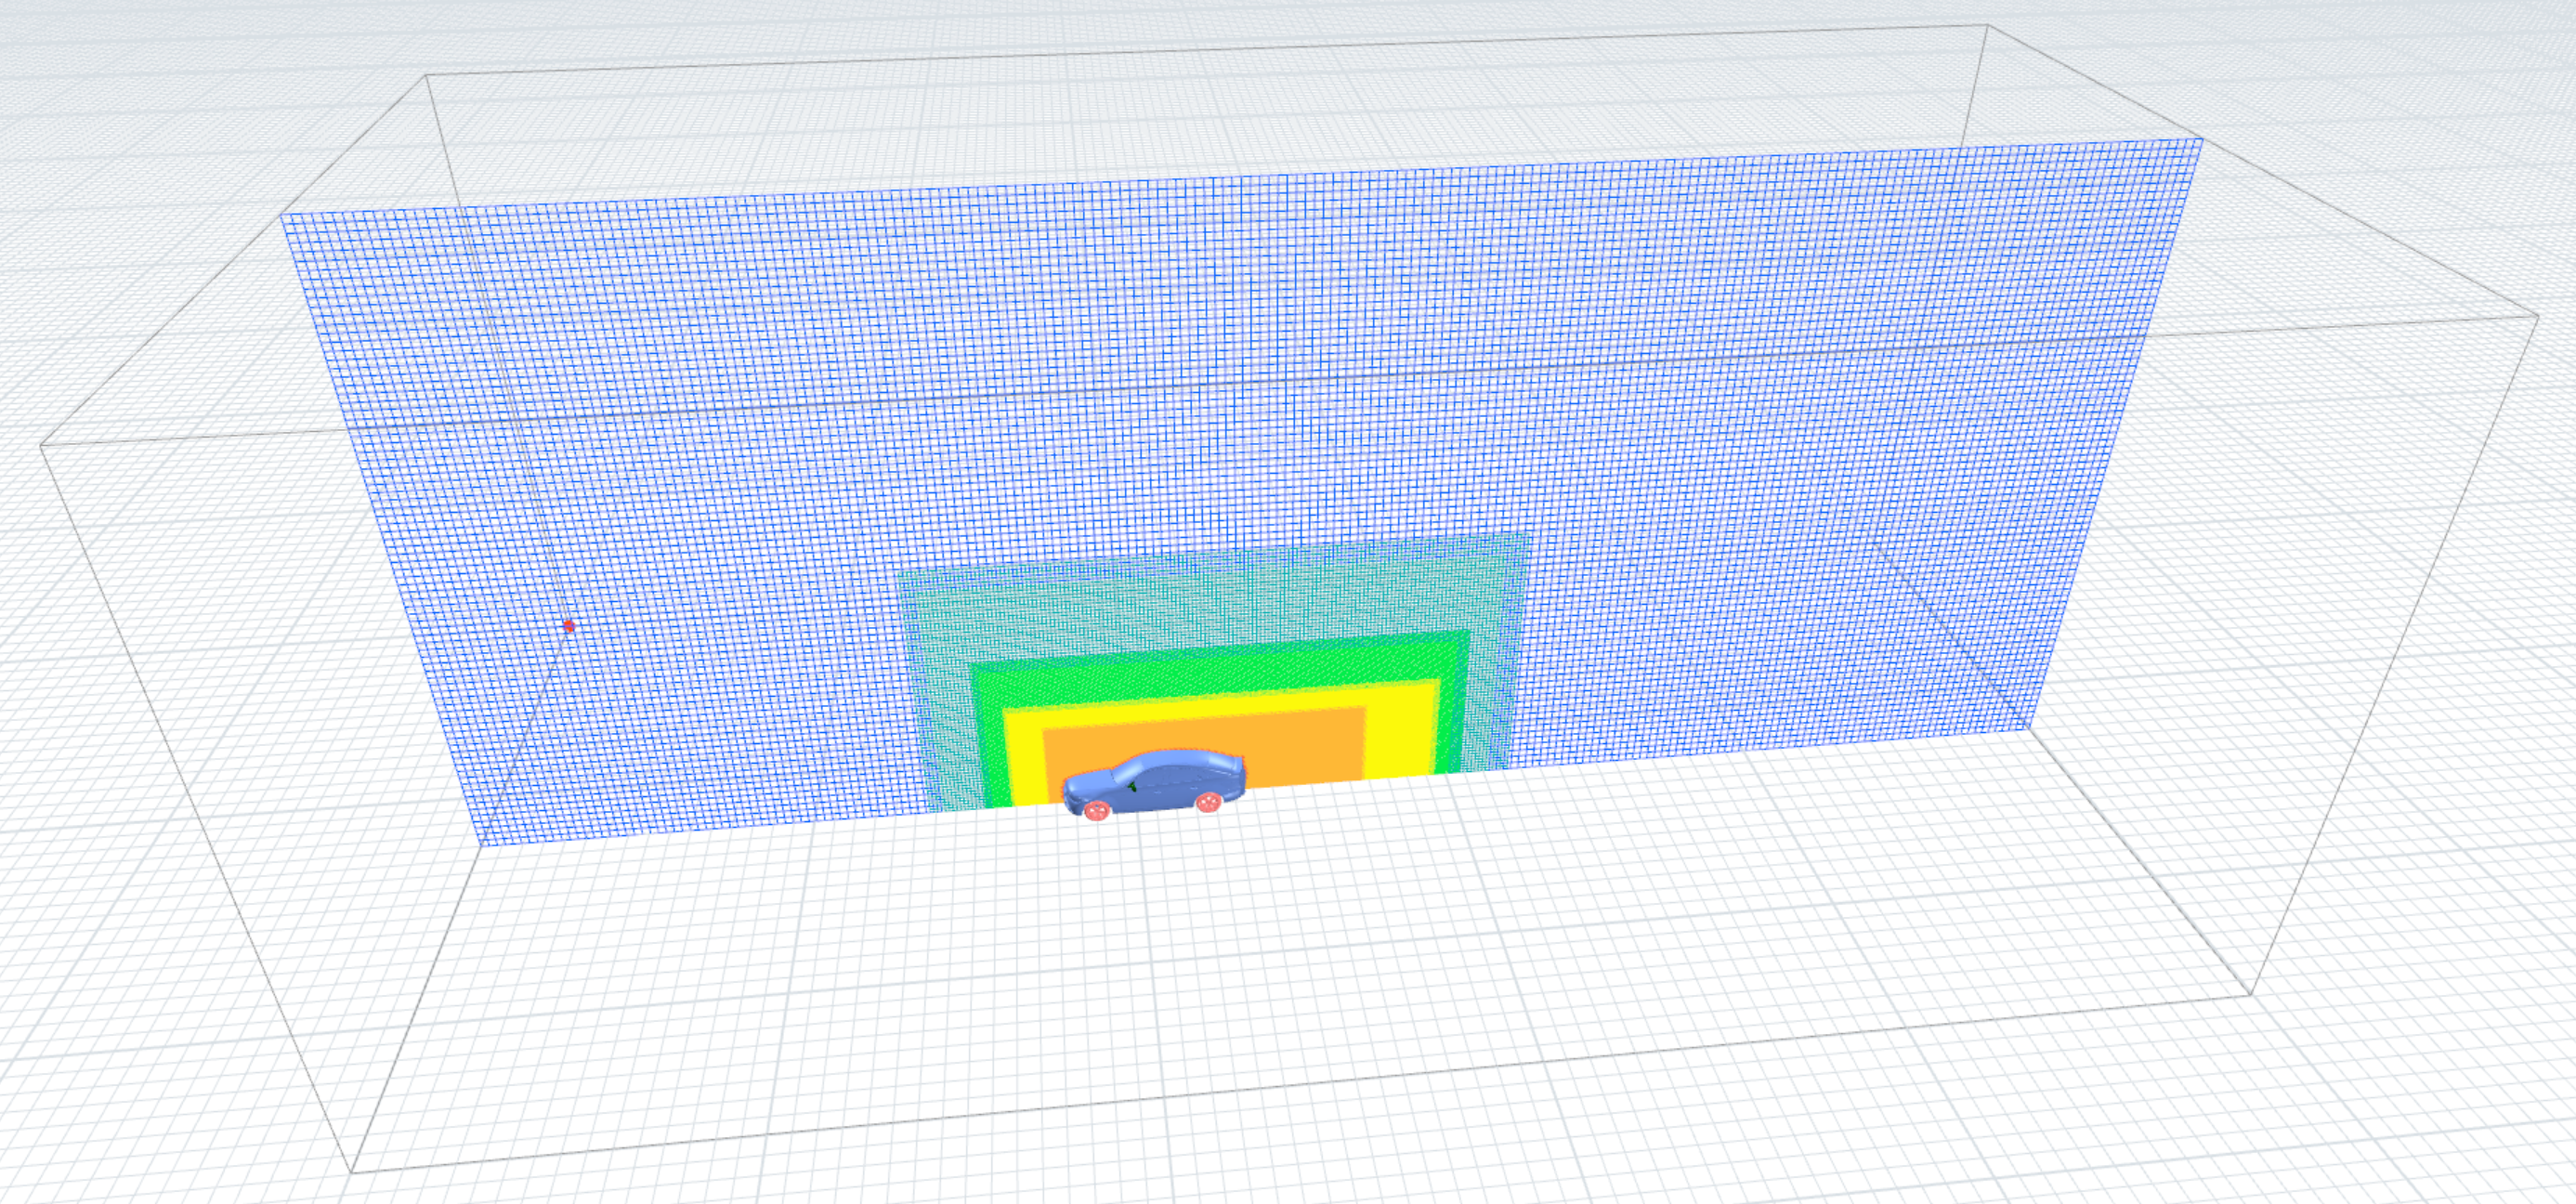
\includegraphics[width=0.99\columnwidth]{figures/domain_setup.png}
  \bicaption[典型的虚拟风洞测试]{典型的虚拟风洞测试。为了准确预测物理量,计算域 (线框中的) 在各个方向的大小应为模型本身的包围盒的约10倍。}{Typical virtual wind tunnel test. For accurate prediction of physical quantities, the computational domain (in wireframe) should have a size typically \~10 times the size of the model's bounding box, in each direction.}
  \label{img:domain_setup}
\end{figure}

为了验证我们的虚拟风洞系统,我们进行了三组对比实验。所有的实验都包含实际风洞的测试结果,以与我们的仿真结果进行定性与定量的对比。这三组实验分别为球的阻力危机、高尔夫球的气动特性与DrivAer标准汽车测试模型的气动特性。下面我们将依次描述这三组实验。

\begin{figure}[htb]
\centering
  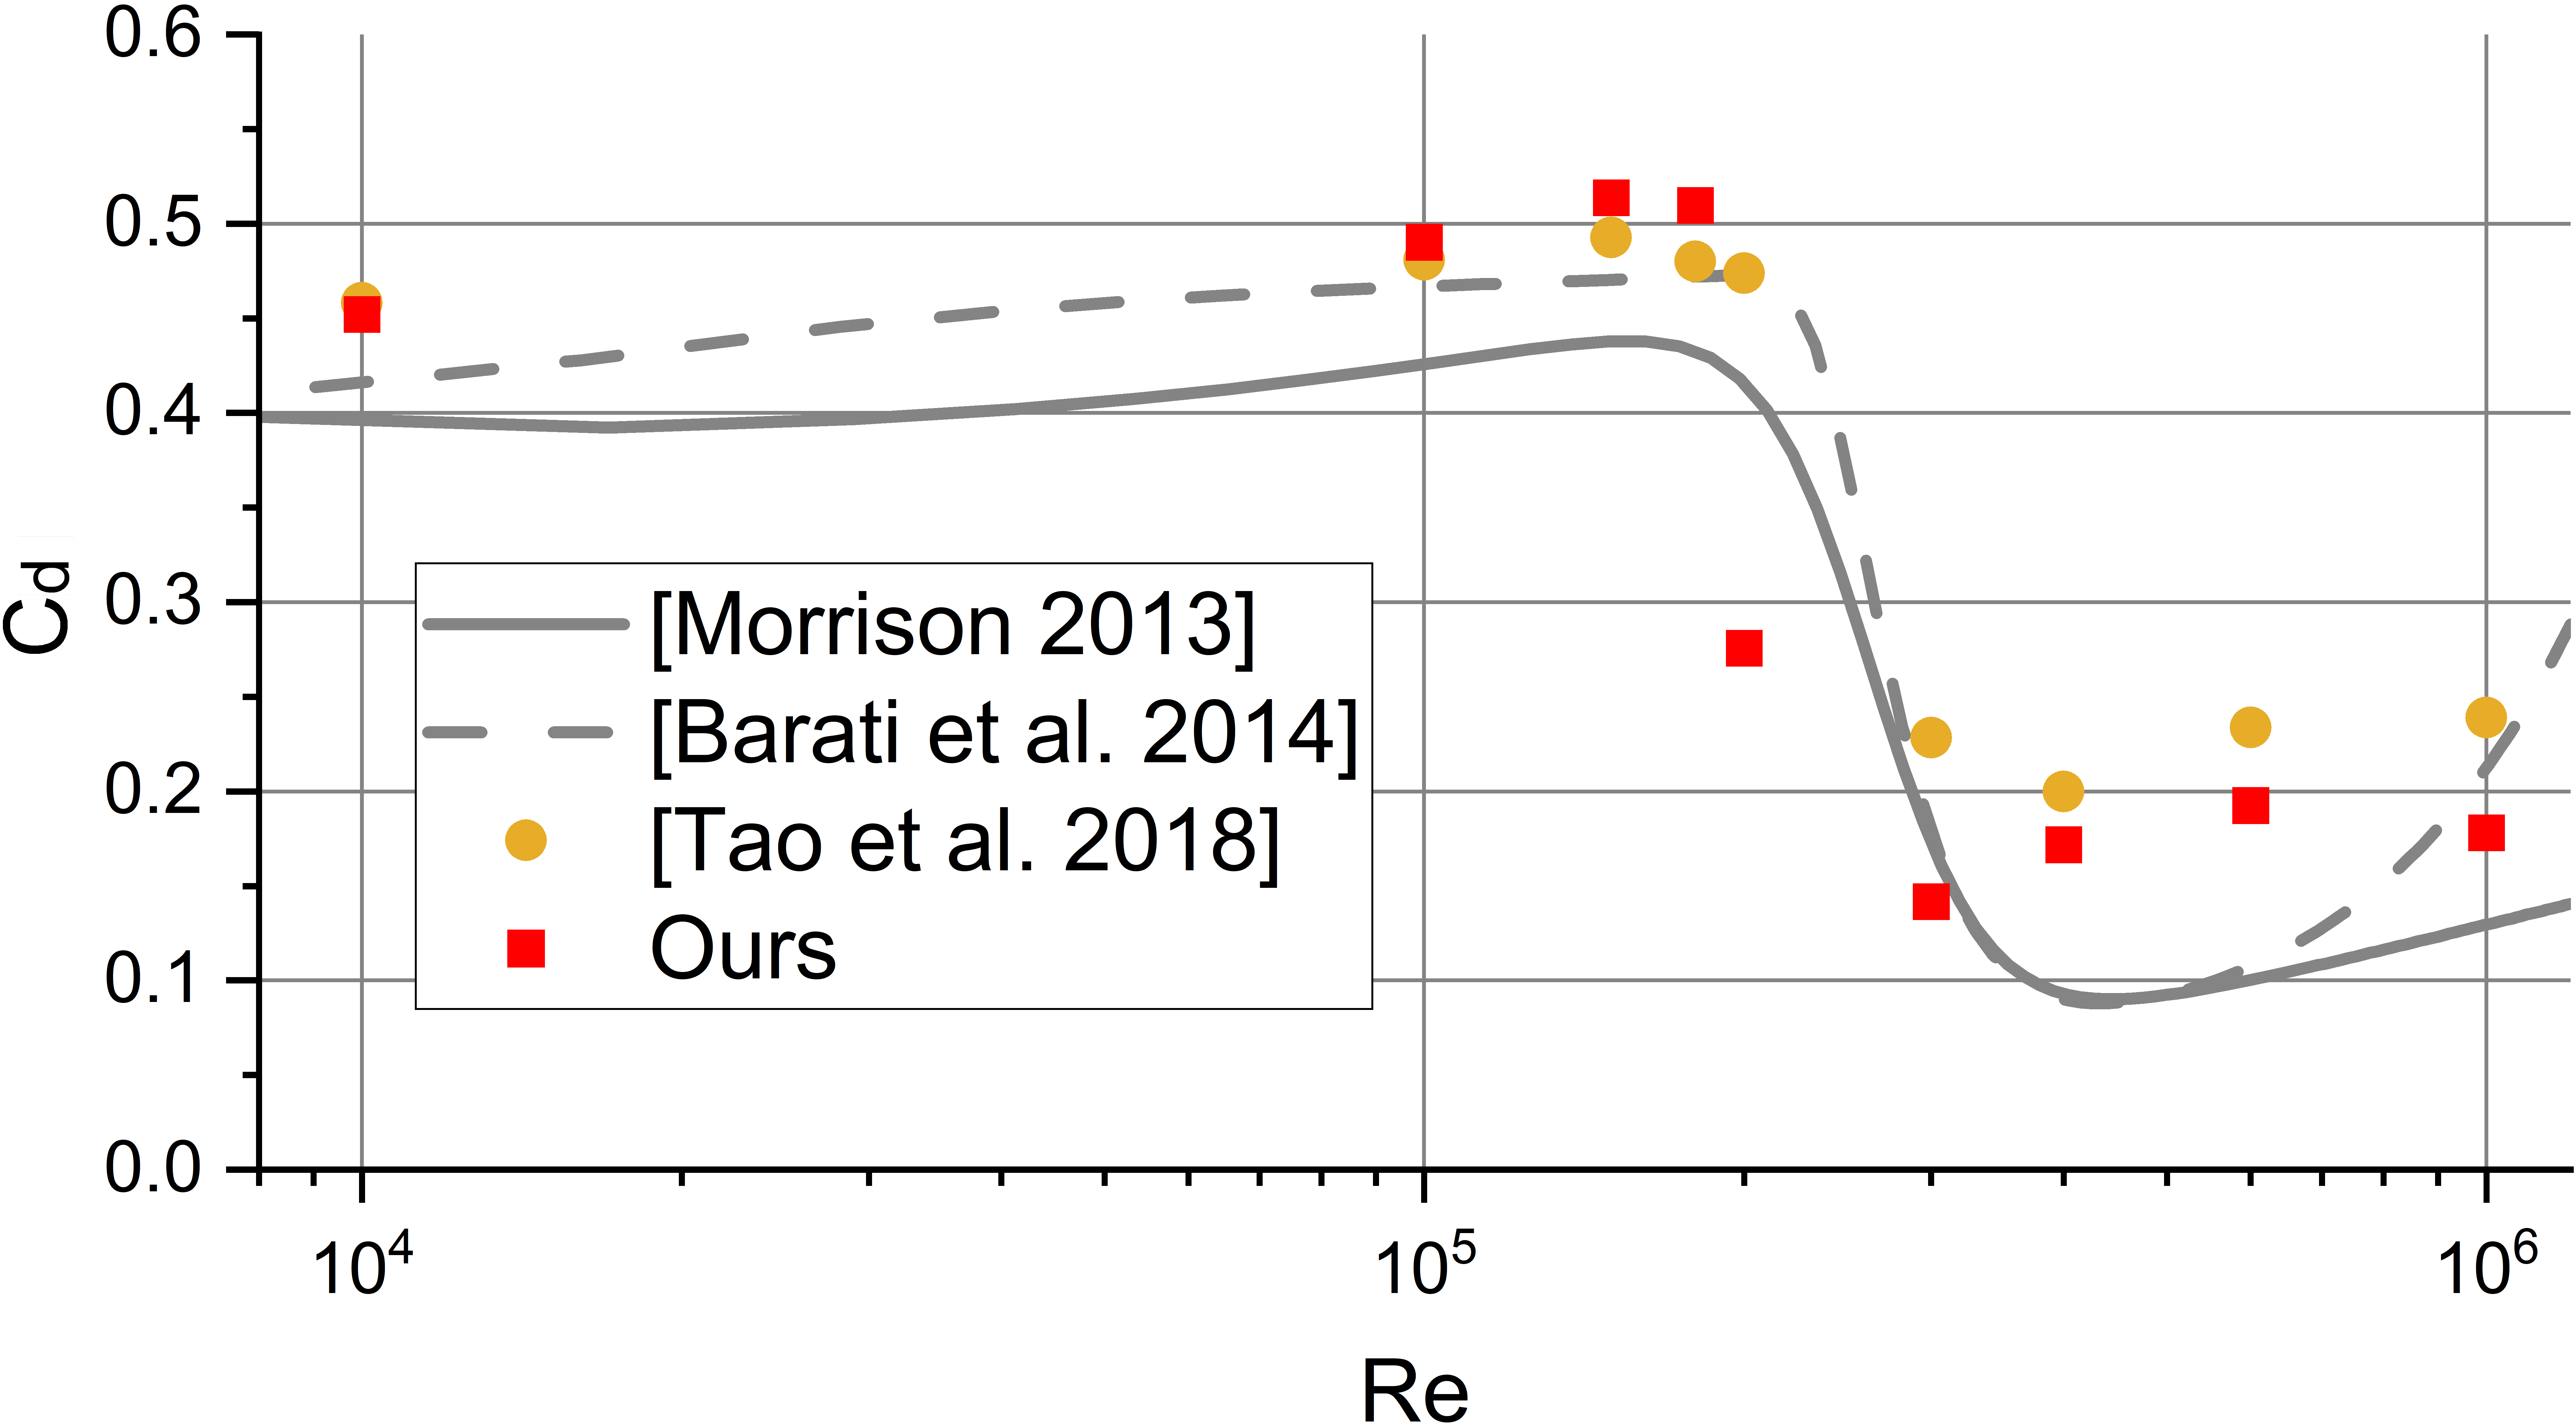
\includegraphics[width=0.75\columnwidth]{figures/sphere_cd_comp.png}
\bicaption[球的阻力与雷诺数的关系]{球的阻力与雷诺数的关系。在我们的仿真中,球在雷诺数在Re=400,000 (阻力危机) 时,\cite{Tao-2018-b} 与我们的方法都展示出了一个突然的阻力下降,之后又稍有上升,与实际实验~\cite{Morrison-2013,Barati-2014} 一致。}{Drag of a sphere vs. Reynolds number. Just like real-life experiments~\cite{Morrison-2013,Barati-2014} exhibit a sudden drop in drag for a sphere at a Reynolds number around Re=400,000 (drag crisis), both \cite{Tao-2018-b} and our kinetic solver demonstrate a similar drop at roughly the same Re, followed by a partial drag recovery.}
\label{img:drag_comp}
\end{figure}

\begin{figure}[htb]
\centering
  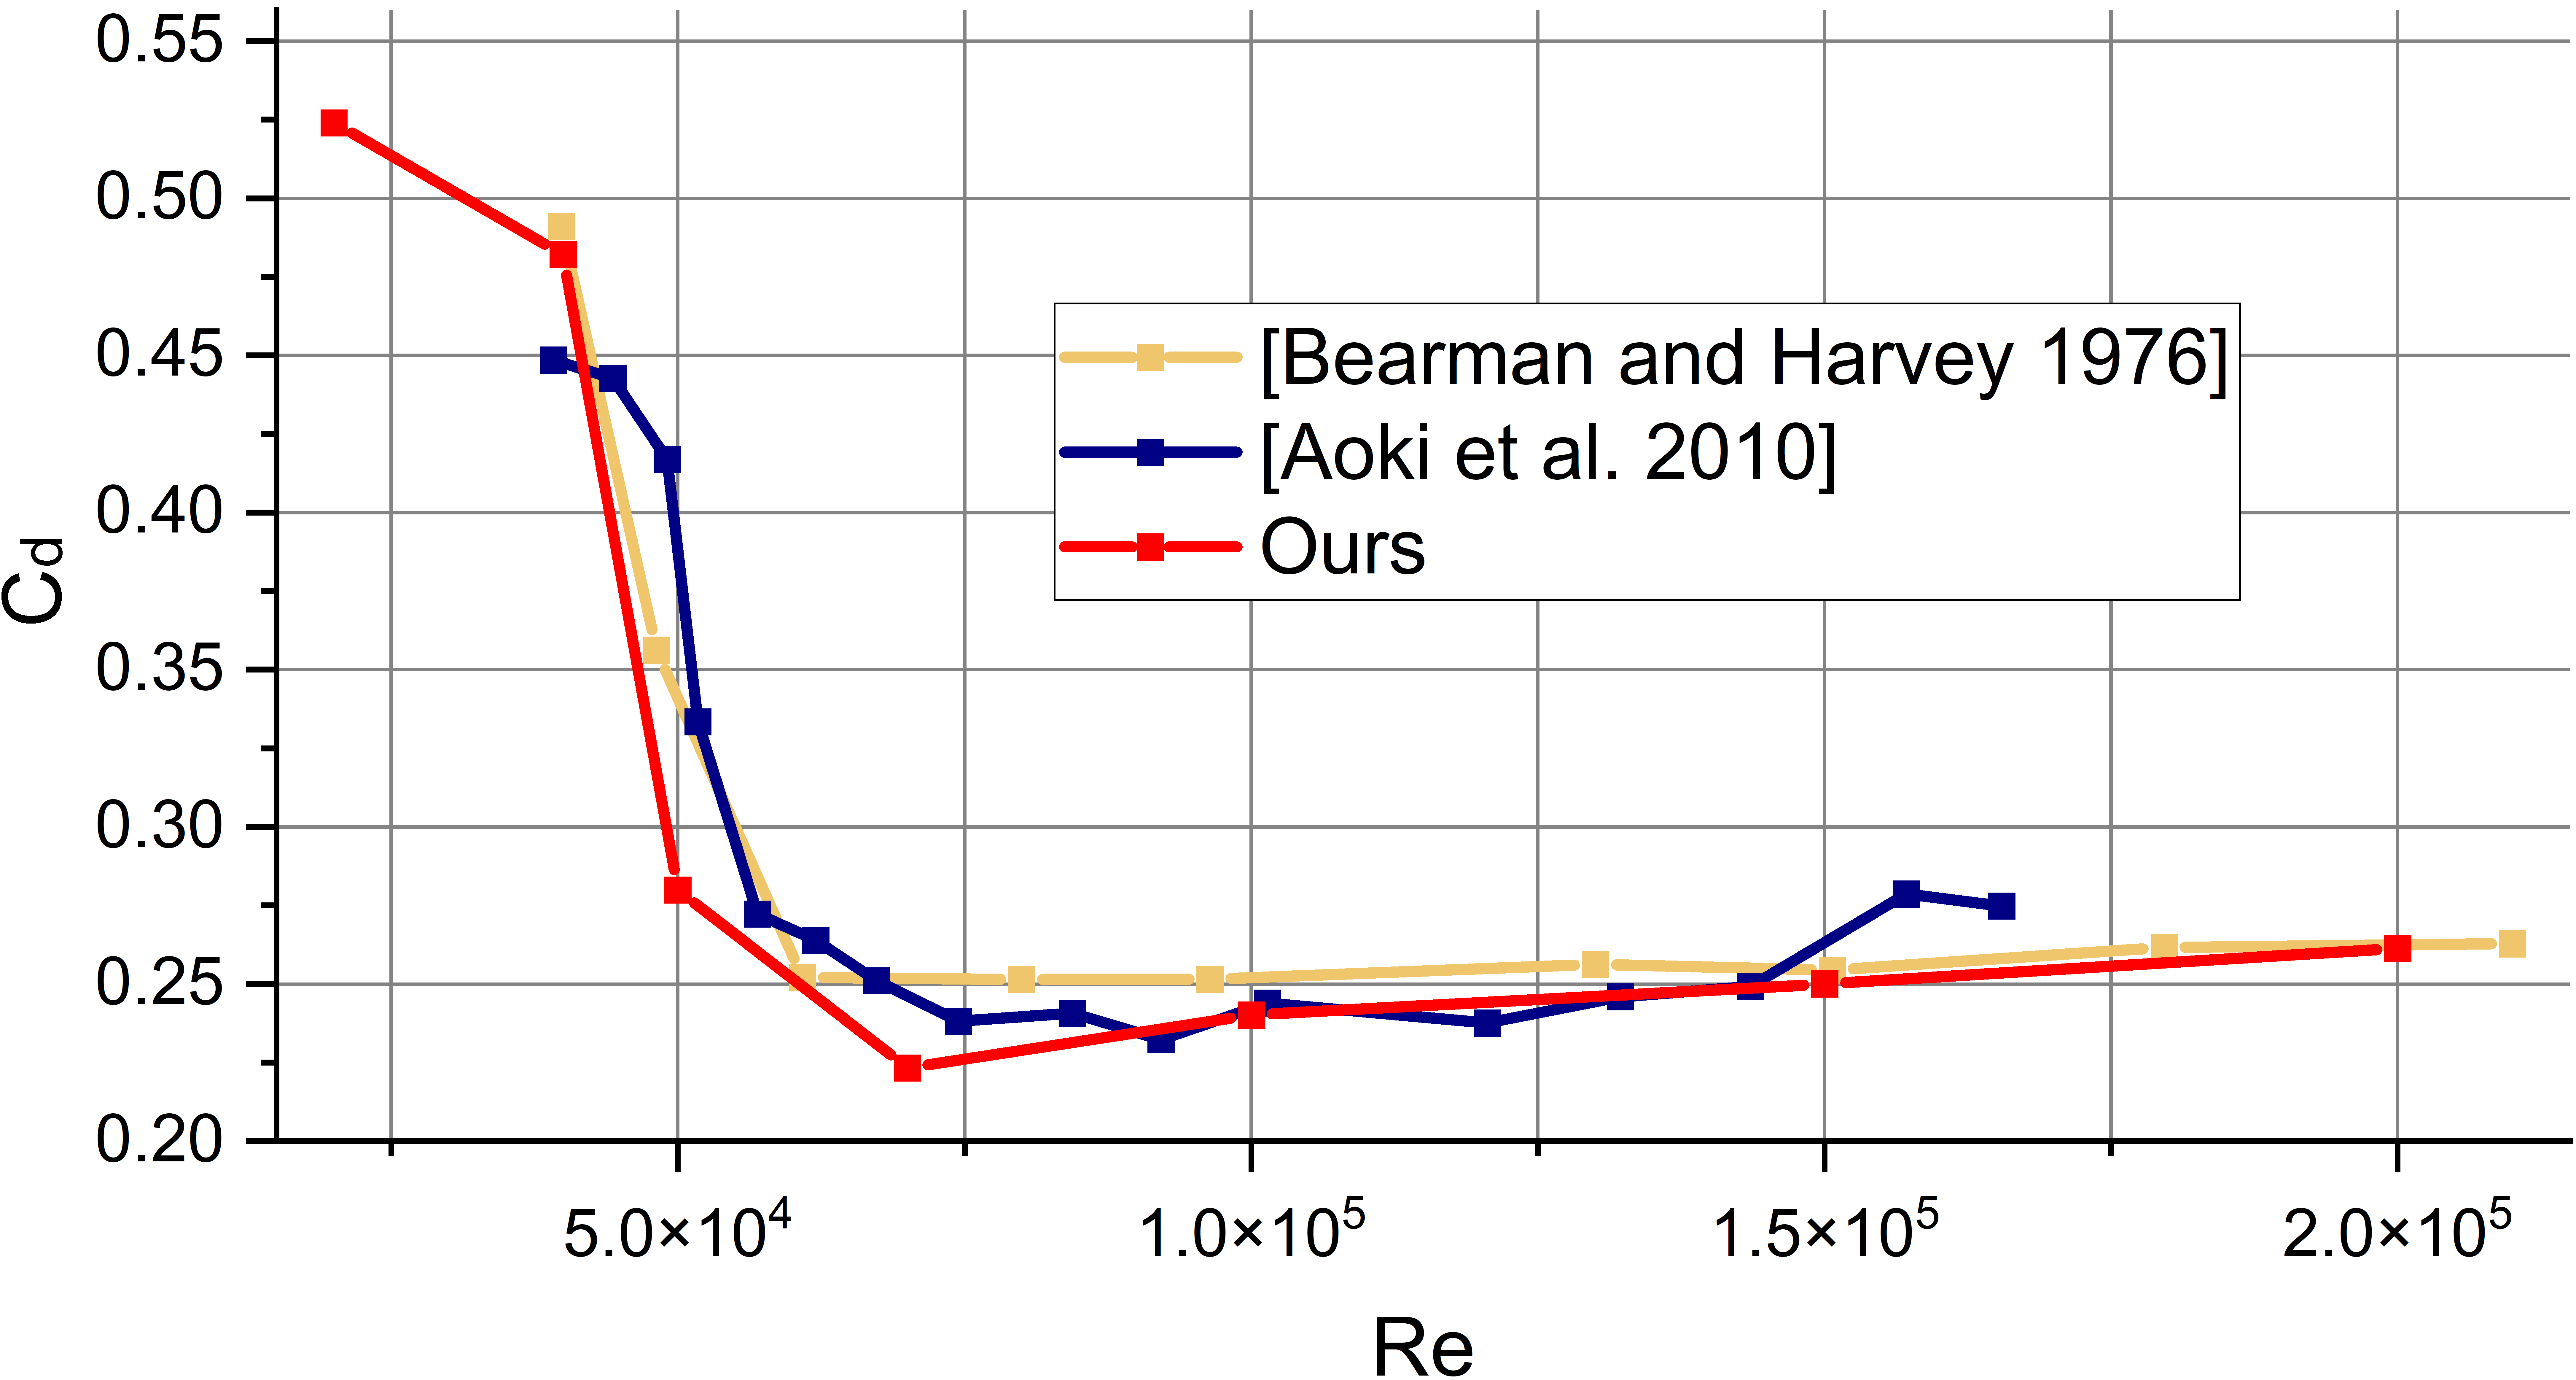
\includegraphics[width=0.88\columnwidth]{figures/golf_ball_cd.png}
\bicaption[高尔夫球的阻力与雷诺数的关系]{高尔夫球的阻力与雷诺数的关系。图中绘制了高尔夫球的阻力系数与雷诺数之间的关系,与真实实验~\cite{Bearman-1976,Aoki-2010} 相比,我们的仿真给出了十分相近的结果。注意高尔夫球阻力突然下降 (阻力危机) 的位置与先前图~\ref{img:drag_comp} 所给出的光滑球相比,雷诺数要小得多。}{Drag of golf ball vs. Reynolds number.Compared to the real-world experiments reported in~\cite{Bearman-1976} and~\cite{Aoki-2010} for the drag coefficient of golf ball as a function of the Reynolds number Re, our wind tunnel simulator provides very similar evaluations. Note that the drop in drag coefficient (drag crisis)  happens far earlier than in the case of a smooth sphere, as expected --- see Fig.~\ref{img:drag_comp}.}
\label{img:golf_ball_cd}
\end{figure}

\begin{figure}[htb]
\centering
  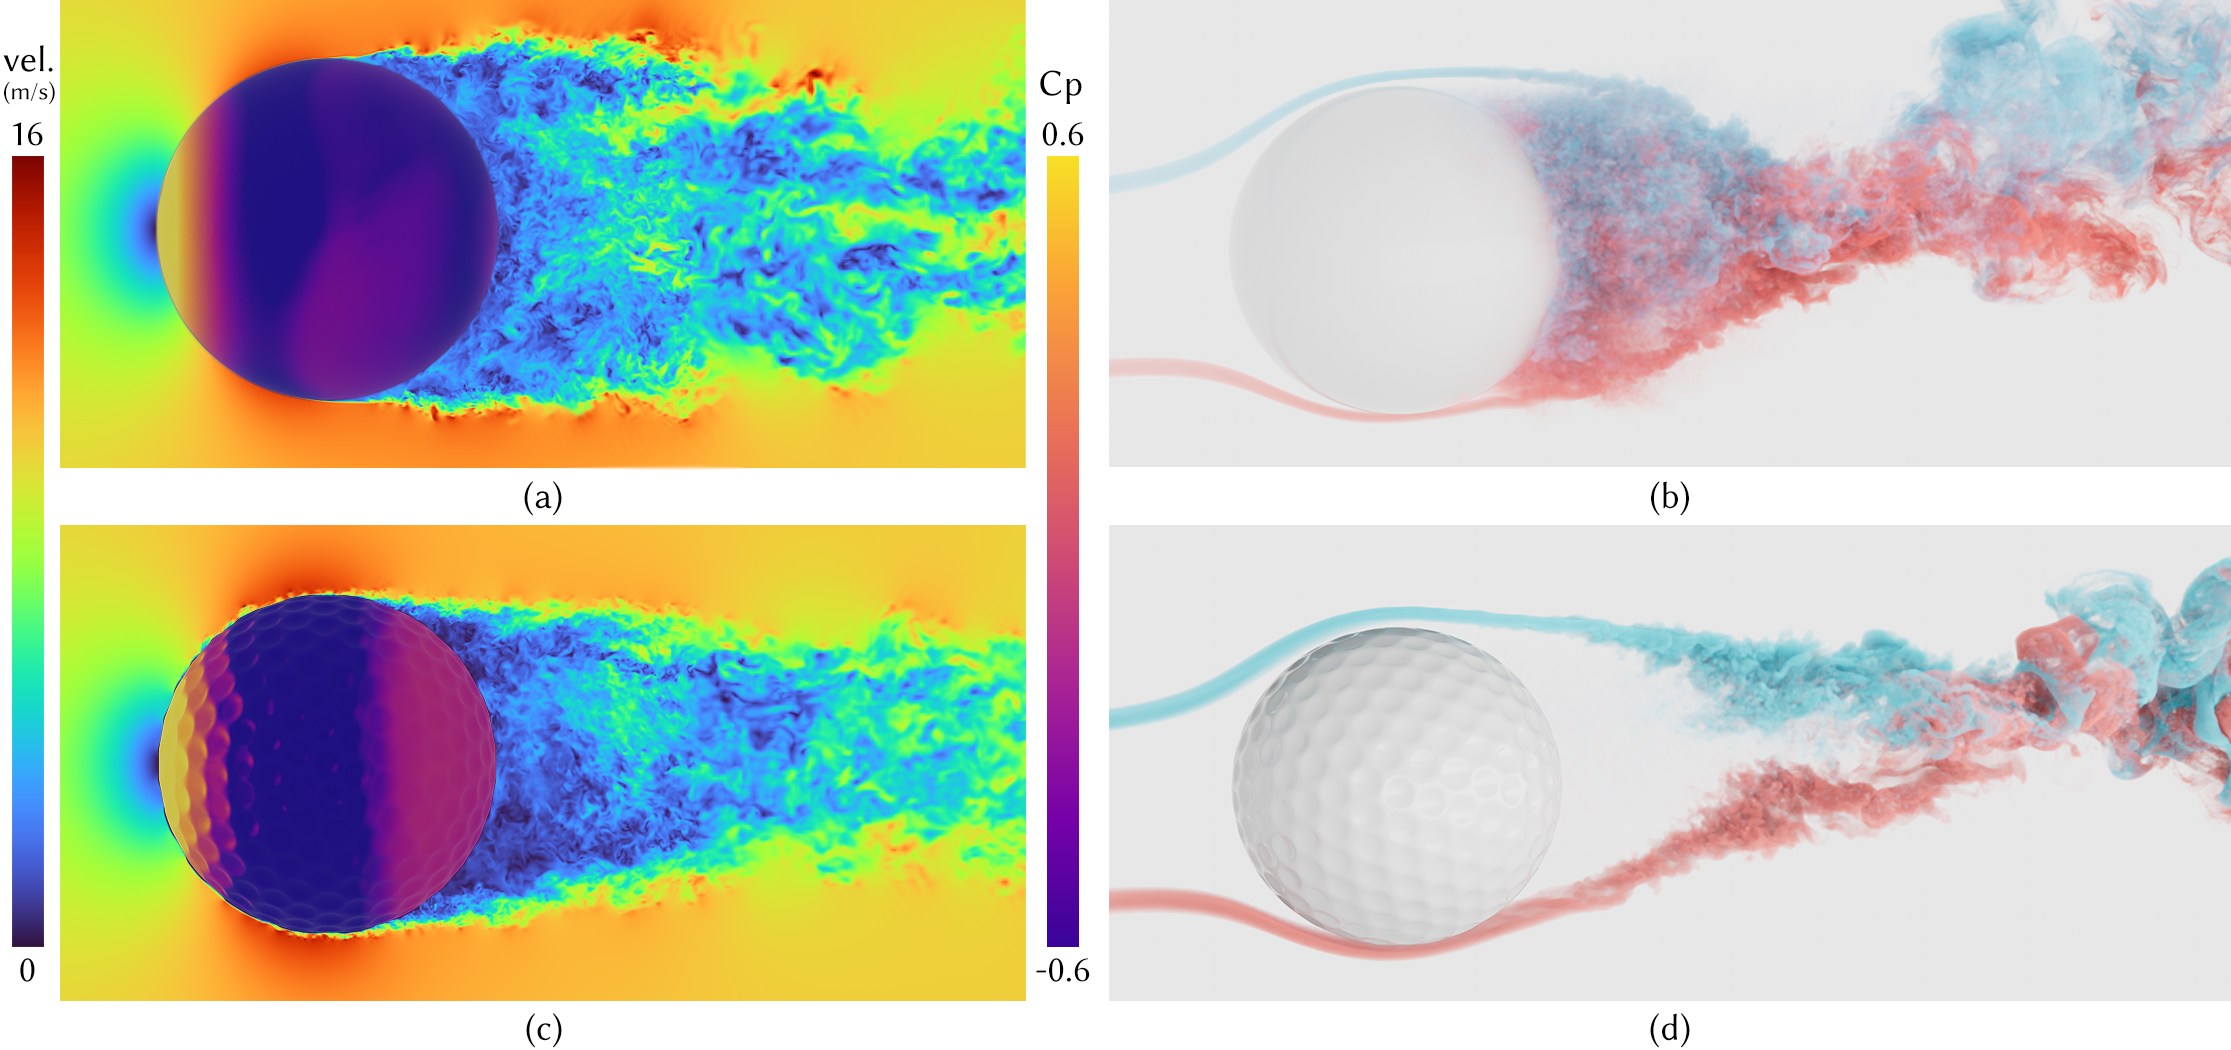
\includegraphics[width=0.99\columnwidth]{figures/golf_ball_vis.png}
\bicaption[光滑球与高尔夫球在Re=100,000时的对比]{光滑球与高尔夫球在Re=100,000时的对比。即使光滑球 (图中顶部子图) 与高尔夫球 (图中底部子图) 大小相同,只有表面的坑洞区别时,在我们的虚拟风洞测试中,也展现出完全不同的速度场与表面压力 ($C_\text{p}$) 场 (左图)。当我们使用染色粒子对流场进行被动追踪时,我们可以更清楚直观地看到这两者尾流所产生的区别 (右图),以理解为什么高尔夫球相对光滑球可以飞得更远。}{Ping-pong vs. golf ball at Re=100,000. While a ping-pong ball (top) differs (up to scale) from a golf ball (bottom) only in the absence of tiny dimples on its surface, testing these two balls in our wind tunnel exhibits very different velocity and surface pressure ($C_\text{p}$) fields (left); consequently, the flows visualized via passively-advected dyed particles are dramatically different (right), providing a good intuition of why golf balls can travel much further.}
\label{img:golf_ball_vis}
\end{figure}

\begin{figure}[htb]
\centering
  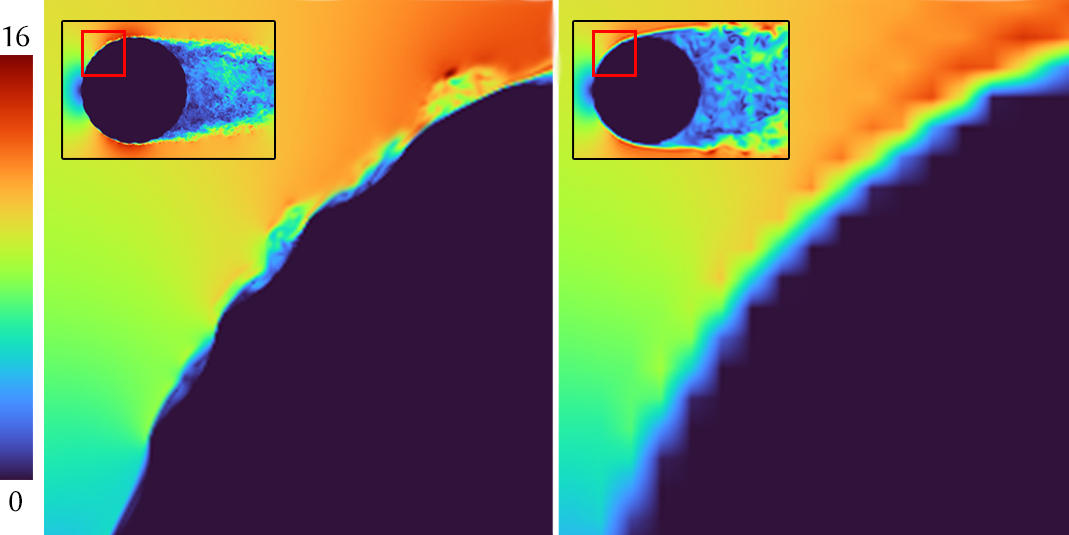
\includegraphics[width=0.9\columnwidth]{figures/golf_ball_single_res.png}
\bicaption[多分辨率网格与单分辨率网格仿真的对比]{多分辨率网格与单分辨率网格仿真的对比。多分辨率网格可以对边界层有更准确的捕捉,在这个例子中可以将高尔夫球表面的小坑洞中的流体准确解算 (左图)。与总格点数相同的单分辨率网格 (右图) 相比,我们可以看到完全不同模式的湍流尾流。图中通过颜色可视化的为速度的模值,单位为$m/s$。}{Multi- vs. single-resolution simulation. A multiresolution simulation better resolves the boundary layer flow going within the small dimples of a golf ball (left), while a single-resolution simulation with the same total number of grid nodes cannot (right). As a consequence, we witness a very different behavior of the turbulent wake when the velocity magnitude (with a colormap indicating its value in $m/s$) is visualized.}
\label{img:golf_ball_comp_single_res}
\end{figure}

\subsection{球的阻力危机}
阻力危机是一个很特殊的空气动力学现象,我们用风吹过球的场景对这一现象进行简单描述。可以想象,球在风中是受到了一定的阻力的,通过实验人们发现这个阻力的大小与雷诺数有关。随着雷诺数的上升,起初阻力没有大的变化。但在到达某一个特定的雷诺数后,球受到的阻力会快速且剧烈地下降。这个雷诺数我们可以称为临界雷诺数。这一现象被成为阻力危机现象。想要在数值仿真中预测这一现象是十分具有挑战性的,尤其在没有湍流模型时,因为这一现象要求求解器对边界层必须求解得足够精准。
需要说明的是,球的阻力危机发生在很高的雷诺数条件下,并且受到实际实验条件限制,精准地获取阻力系数也是十分困难的。所以在我们参考的实际实验数据中~\cite{Morrison-2013, Barati-2014},不同的实验数据也有一定的差异。而图~\ref{img:sphere_wake_comp} (c) 中的实验可视化是通过在球上添加了一个额外的环来增加有效雷诺数,从而在低雷诺数环境中进行的等效实验。

我们的虚拟风洞系统可以定性地重现阻力危机这一现象 (见图~\ref{img:drag_comp}),即在正确的临界雷诺数,球受到的阻力产生明显且剧烈的下降。并且相比使用~\cite{Tao-2018-b} 的LBM求解器,我们的方法在临界雷诺数及之后的范围中预测的阻力系数更接近实验值。
我们注意到,我们预测出的阻力在临界区域中与实验值相比有一个小的偏移,使得在Re=200,000时我们的预测结果与实验值有一个较大的偏差。关于这一点,我们需要说明的是,即使是实际实验中,阻力系数也是在剧烈变化的。我们这里列出的实验获得的阻力系数值可以被认为是一个时间段内的平均。在这样一个流体正在发生从临界雷诺数前到临界雷诺数后转变的过程中,数值仿真得到的阻力系数也有着剧烈的抖动。在这样一个位置无论是实际实验,或数值仿真,进行准确的预测都是十分困难的。关于这一点,在~\cite{Geier-2017-b} 中有非常详尽的讨论。
我们同时注意到,我们的方法在临界雷诺数后的区域,对阻力的预测过大。实验值显示该区域的阻力系数$C_\text{d}$约为0.1,而我们的方法预测在$0.175$附近,但好于~\cite{Tao-2018-b} 中预测的$0.2$。由于这一区域是在极高的雷诺数下,通过直接数值仿真来准确求解边界层,对于现有的流体求解器,均是十分困难的~\cite{Tiwari-2020}。

\subsection{高尔夫球的气动特性}
我们还在虚拟风洞中测试了高尔夫在高速气流下的气动特性。我们使用的高尔夫球模型有362个坑洞 (美国职业高尔夫球巡回赛的赛事用球拥有最低322个,最高376个坑洞),坑洞深度与球的直径的比值为0.007。
如图~\ref{img:golf_ball_cd},我们通过仿真得到的阻力系数与已发表的实验数据~\cite{Bearman-1976, Aoki-2010}相吻合。这个结果同时可以验证我们的方法对于小尺度的几何变化的敏感性。在Re=100,000时,高尔夫球与表面光滑的球所造成的尾流截然不同。原因在于高尔夫球表面的小坑洞可以产生非常小的边界层涡流,并影响周围的流场,减小层流边界层在固体边界上的附着,这使得高尔夫球表面流场的分离点相比平滑球将更靠后,形成更加收窄的尾流形状,并降低自身阻力。这一点可见图~\ref{img:golf_ball_vis}。
注意我们的多分辨率网格是能捕捉到这样的小细节的关键。如果我们采用单分辨率网格,即使总网格数相同,也没有能力捕捉到高尔夫球表面坑洞所造成的薄边界层。这会造成仿真错误地预测边界分离点与尾流形状,并得到大幅升高的阻力系数,见图~\ref{img:golf_ball_comp_single_res} (右)。

\begin{figure}[!htbp]
  \centering
    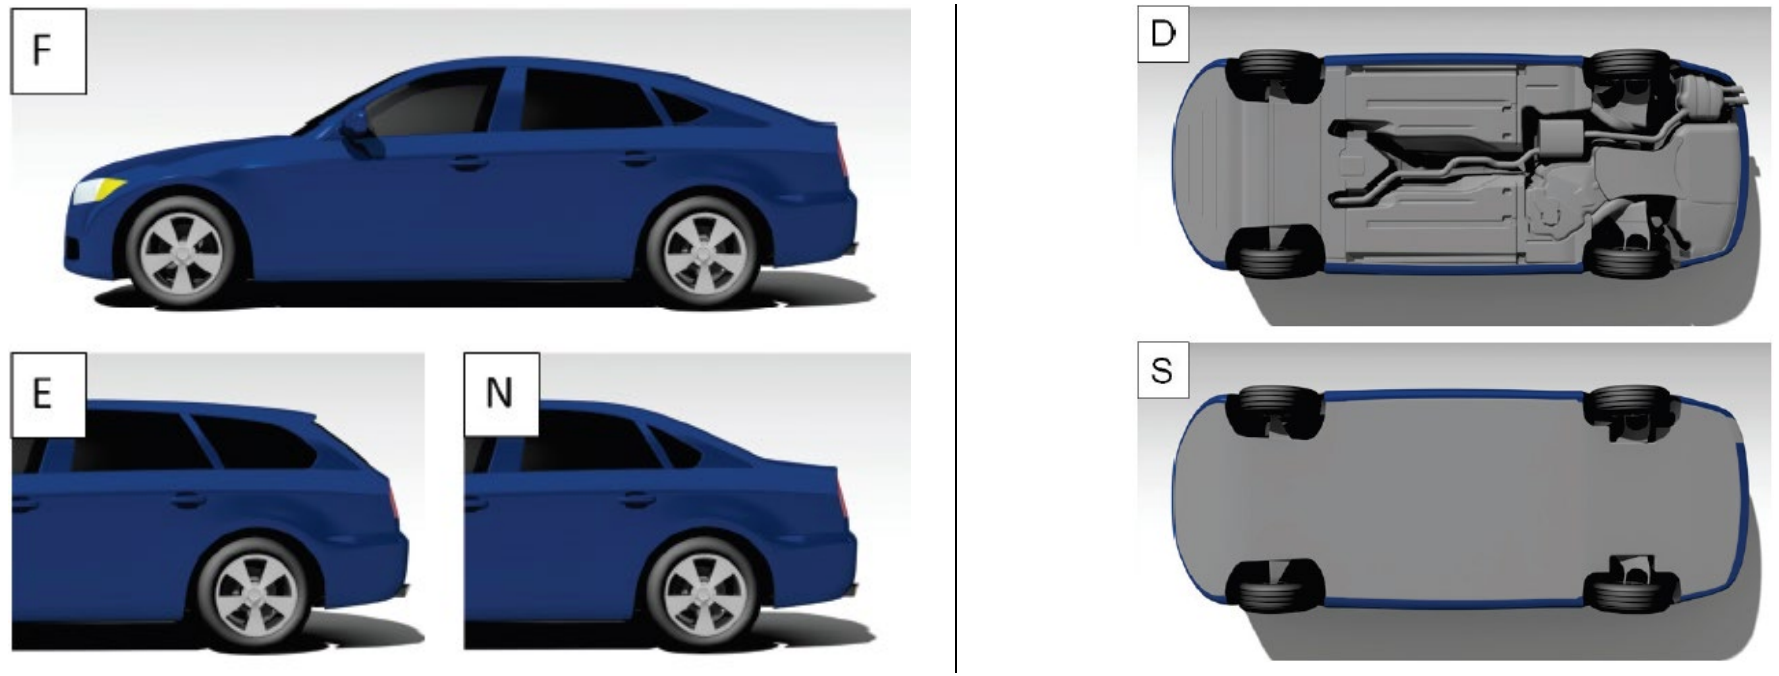
\includegraphics[width=0.99\columnwidth]{figures/drivaer_model.png}
  \bicaption[DrivAer模型尾部和底盘的不同配置]{DrivAer模型尾部和底盘的不同配置。尾部的配置 (左图):快背式 (F)、阶背式 (E) 与方背式 (N)。底盘的配置 (右图):复杂底盘 (D) 与平滑底盘 (S)。图片来自~\cite{deltransient}。}{Rear end and underbody configurations of DrivAer. Rear end configurations (left): fastback (F), estate back (E) and notchback (N). Underbody configurations (right): detailed (D) and smooth (S). Image from~\cite{deltransient}.}
  \label{img:drivaer_model}
\end{figure}

\begin{figure}[!htbp]
  \centering
    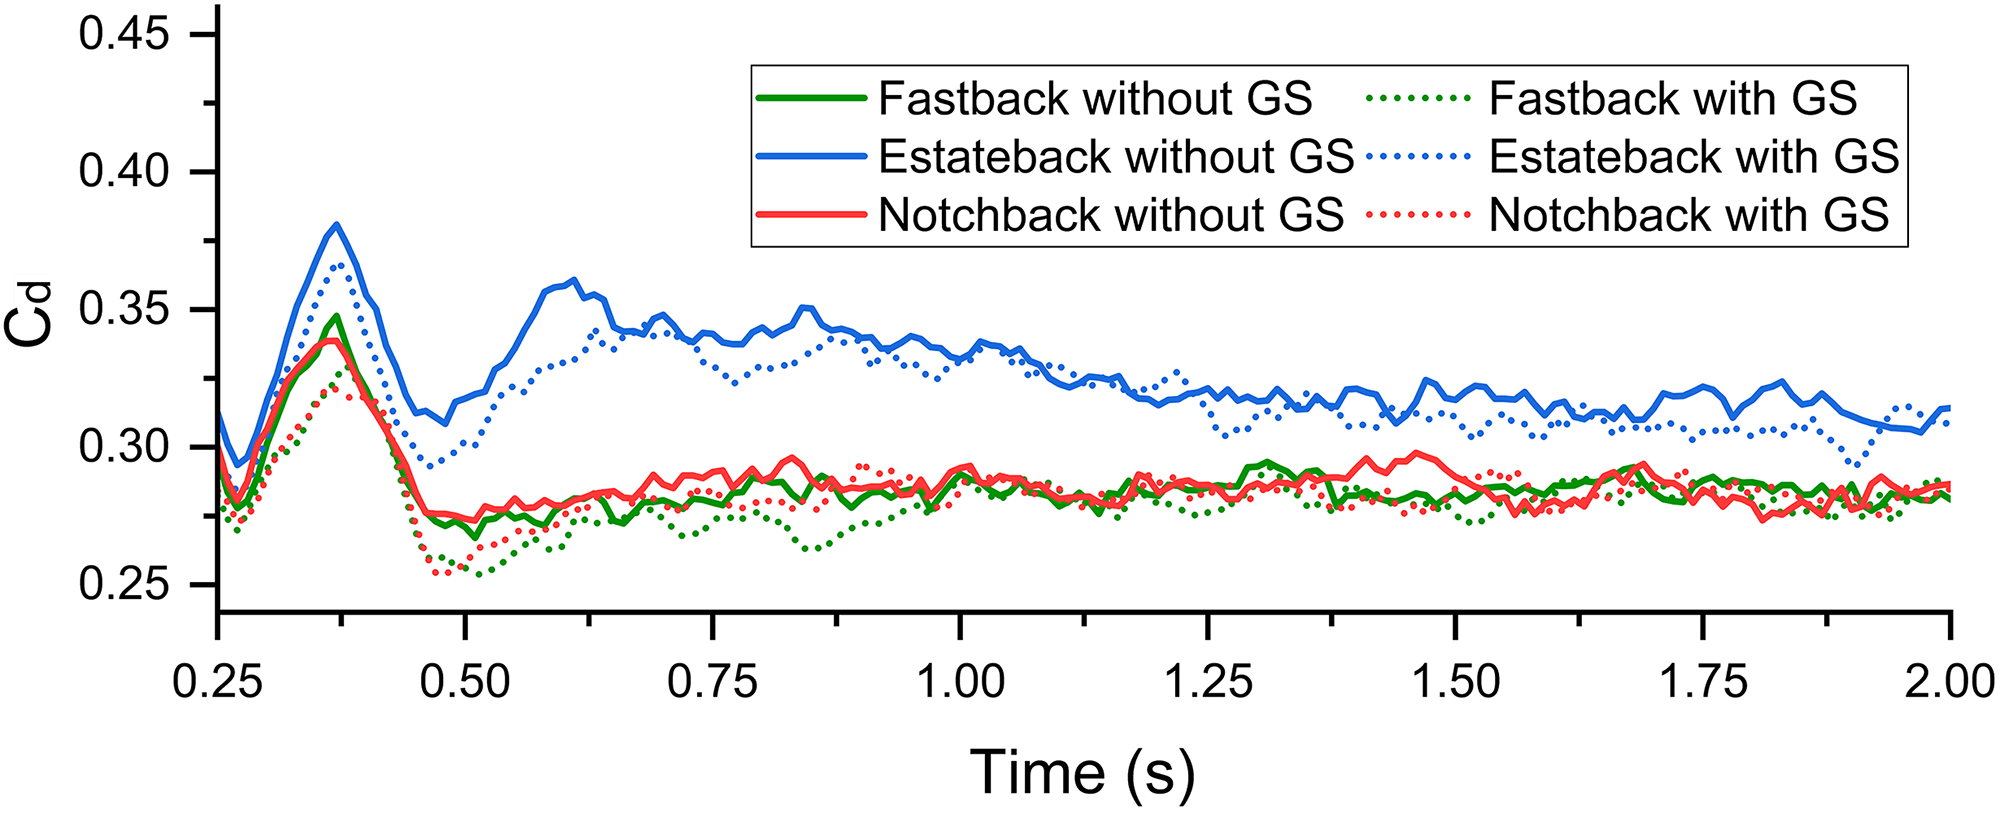
\includegraphics[width=0.9\columnwidth]{figures/tum_validation_cd_curve.png}
  \bicaption[DrivAer汽车的阻力随时间的变化]{DrivAer汽车的阻力随时间的变化。我们画出我们仿真所给出的不同DrivAer汽车配置的阻力系数随时间的变化,包括有地面仿真与无地面仿真的情况。(GS表示有地面仿真,即汽车的轮胎旋转且地面运动的速度与轮胎的线速度一致。)}{Car drag over time. We plot the simulated drag coefficient in time for different DrivAer car configurations, with or without ground simulation (GS, meaning ground motion and rotating wheels are simulated).}
  \label{img:tum_validation_cd_curve}
\end{figure}
  
\begin{figure}[!htbp]
  \centering
    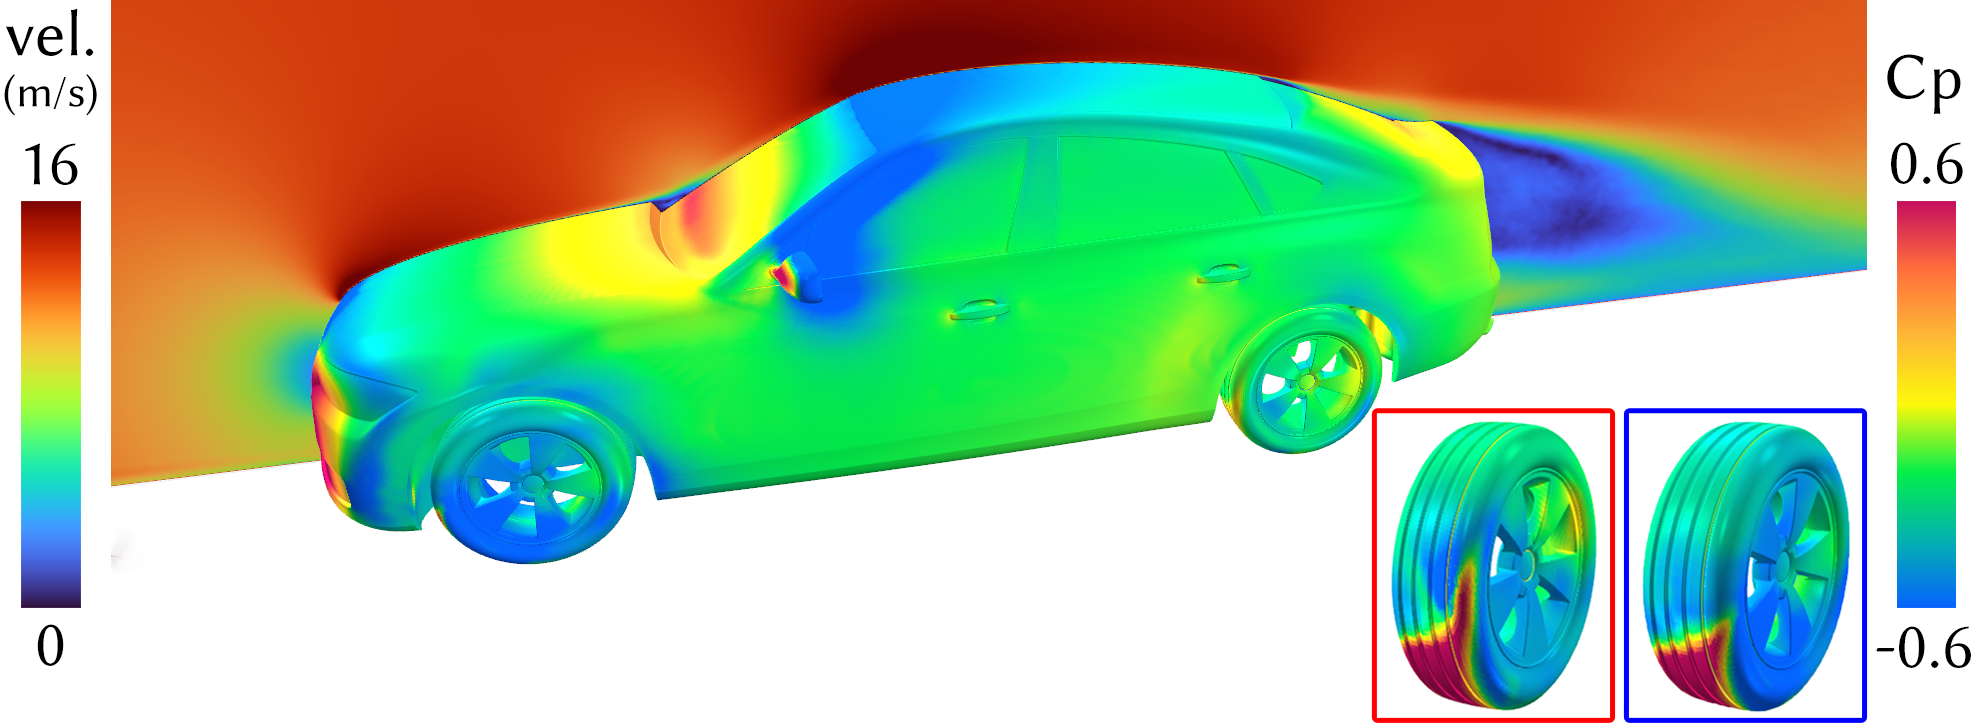
\includegraphics[width=0.9\columnwidth]{figures/tum_fastback.png}
  \bicaption[DrivAer fastback汽车的空气动力仿真]{DrivAer fastback汽车的空气动力仿真。我们对DrivAer fastback这样的标准测试车型进行气动仿真,图中展示了垂直的平均速度场截面,与模型表面的平均压力 (平均均指随时间平均)。轮胎在有地面仿真 (蓝色方框内) 与无地面仿真 (红色方框内) 时的平均表面压力可视化也在图中展示。}{DrivAer Fastback aerodynamic simulation.
  A vertical cross-section shows the magnitude of the mean velocity flow around the DrivAer fastback benchmark car model, while the mean pressure over the model surface colors the mesh.
  Mean pressure distributions without (red inset) and with (blue inset) ground simulation are also visualized on the wheels.}
  \label{img:fastback}
\end{figure}
  
\begin{table}[!htbp]
    \centering
  \bicaption{DrivAer汽车模型的阻力计算精度。我们对我们仿真得到的不同DrivAer车型配置的阻力系数$C_\text{d}$与实验值进行了比较。GS表明地面仿真,即有GS时地面运动且轮胎旋转。}{Drag estimation accuracy of DrivAer car model. We compare our estimates of the drag coefficient $C_\text{d}$ for different DrivAer configurations with experimental data, with or without ground simulation (GS, meaning ground motion and rotating wheels are simulated).}
  \begin{tabular}{*{4}{c}}
        \toprule
    车型配置 & 仿真所得$C_\text{d}$ & 实际实验所得$C_\text{d}$ & 相对误差 \\
        \midrule
    快背式 (无GS) & 0.2849 & 0.284 & 0.32\%\\
    阶背式 (无GS) & 0.2851 & 0.286 & -0.31\%\\
    方背式 (无GS) & 0.316 & 0.318 & -0.63\%\\
    快背式 (有GS) & 0.2811 & 0.275 & 2.22\%\\				
    阶背式 (有GS) & 0.283 & 0.277 & 2.17\%\\				
    方背式 (有GS) & 0.3089 & 0.319  & -3.17\%\\
        \bottomrule
  \end{tabular}
  \label{tab:drivaer_result}
\end{table}

\subsection{DrivAer汽车模型的气动特性}
最后,我们对DrivAer汽车模型进行气动仿真。DrivAer汽车模型是慕尼黑工业大学 (Technische Universit\"at M\"unchen) 所制造的一个标准汽车测试模型,其主要目的是为了研究汽车外形对空气动力学特征的影响,同时验证数值仿真算法的能力~\cite{Heft-2011, Heft-2012}。这一模型在汽车工业受到广泛认可。

我们在测试中使用了三种不同的车型配置,三种配置的主要区别是汽车尾部的造型区别,分别被称为快背式 (fastback)、阶背式 (notchback) 与方背式 (estateback),三种配置的几何示意可见图~\ref{img:drivaer_model}。我们在测试中使用的模型的几何精度为3mm,带有发动机盖、轮胎、轮腔、后视镜与复杂底盘,且不考虑发动机舱内的流动。
所有的测试中,气流的流速 (即车速) 都被设置为$57.6 km/h$。并且,对每一个车型配置,我们都测试了有和无地面仿真 (ground simulation, GS) 这两种情况。在有地面仿真的情况中,地面的速度是与车速等同的,且轮胎也在以同样的线速度旋转。而没有地面仿真的情况中,地面和轮胎都维持静止。
这两种情况可以很直观地显示出,轮胎与地面的速度差别,对于风洞实验与气动结果的影响是巨大的。

我们将仿真得到的阻力数据画在了图~\ref{img:tum_validation_cd_curve} 中,这里阻力是随时间变化的。从图中可以看出,在流场经历过初始化带来的不稳定阶段后,阻力在约1 s后趋于稳定。我们将$1.2s$至$2s$区间内的阻力系数平均来得到相应车型配置的阻力系数,并于实际风洞实验值~\cite{Heft-2012b} 相对比,得到的结果可见表~\ref{tab:drivaer_result}。
注意我们的仿真结果是经过了一次平均值修正后的结果。平均值修正即我们将所有仿真结果与对应实验值误差的平均值减去,这样我们得到的可以认为是误差的变化趋势。这是工业设计中一个常见的做法。因为对于汽车这样的复杂模型,数值实验存在系统的偏差,包括我们之前讨论的地面与车身之间的流场,都会使计算得到的物理量发生整体的偏移。通过平均值修正我们可以弥补这种偏移。
图~\ref{img:fastback} 中展示了平均速度与压力场,平均的时间区间同样为$1.2s$至$2s$。图中分别展示了静止与旋转轮胎的表面压力,以显示有地面仿真和无地面仿真时的区别。
与我们的预想相一致,在没有地面仿真时,我们的方法精度更高,所得结果的误差平均约为$0.4\%$。这一结果远小于工业仿真中通常要求的$3\%$误差标准 (这一误差标准是我们与汽车制造商沟通获得的)。在有地面仿真时,我们的最大误差为$3.17\%$,也足以满足工业仿真中的需求 (在有地面仿真时,误差标准可以更宽容,一般在$5\%$)。

\paragraph{与现有工业软件的对比}
目前有许多商业的工业流体仿真软件,与我们的虚拟风洞系统所描述的功能类似。其中西门子 (Siemens) 的StarCCM+~\cite{Siemens} 与达索 (Dassault Syst{\`e}mes) 的PowerFLOW~\cite{powerflow}是两个较有代表性且被广泛使用的商业流体仿真分析软件,并分别通过基于FVM的N-S求解器与LBM求解器实现流体仿真。两者一般都运行于CPU集群环境。
因为StarCCM+在进行非稳态仿真时,计算量非常大,仿真时间可达数周,所以StarCCM+更经常被用于稳态求解。而稳态求解的问题是,如面对轮胎旋转这样的场景时,边界必须采取一定的近似。这与实际的物理情况并不相符。PowerFLOW克服了这些问题,但是只能在CPU集群上使用限制了LBM方法的并行优势。
而我们的方法既继承了动理学方法的优势 (即PowerFLOW软件的优势),同时又可以在GPU上解算,使得硬件需求大幅下降。如我们使用NVIDIA A100 GPU (拥有6,912个CUDA核) 对DrivAer的快背式模型进行2s的仿真,在没有地面仿真时只需约3个小时即可完成仿真,即每秒的仿真需要10,356 GPU核时。
James等~(\citeyear{James-2018}) 使用PowerFLOW与StarCCM+分别对DrivAer的方背式模型进行了类似的仿真。在结果达到收敛时,PowerFLOW的仿真在96个CPU的集群上需要约80小时,StarCCM+在128个CPU的集群上需要约13小时。
假设上述CPU拥有至少8个核心的情况下,通过计算我们可以得知在核数相当时,我们的方法是更高效的。当然因为CPU平台与GPU平台直接比较性能是很困难的,我们这里只非常定性地对效率进行了描述。
此外,更引人注目的是,在James等~(\citeyear{James-2018}) 所报告的PowerFLOW的计算结果中,并没有显示出有地面仿真与无地面仿真时,阻力系数有明显区别。这与实验数据相违背。其它的结果与实验值~\cite{Heft-2012b} 相对比时,大约均在3\%的误差水平。
我们需提请注意的是,在该工作中,作者使用了没有后视镜的模型,而我们使用了带有后视镜的模型。此外作者没有提供任何数值修正相关的信息。
这证明了在DrivAer测试中,精度层面上,我们与现有的工业软件是大致相当的。当然我们也认为我们需要与PowerFLOW与StarCCM+等软件进行更直接的对比,以更明确地确定我们的方法与现有工业软件的优劣。这些我们留在未来的工作中。

\section{气动声学的仿真结果}
\subsection{起落架模型的气动声学仿真}
了解和预测民航客机机身的噪声对于提升民航客机的舒适度非常重要。由于高涵道比发动机的使用大大降低了发动机噪音,起落架和增升裝置的噪音开始受到关注。具体地讲,在客机进近时起落架会放出,此时起落架发出的声能 (acoustic energy) 约占飞机总声能的三分之一。除了实际风洞试验,计算气动声学为更好地了解噪声产生机制提供了一条很有前景的途径。在此背景下,由空中客车 (Airbus) 提供支持的LAGOON (LAnding-Gear nOise database for CAA validatiON) 项目尝试提供一个行业标准的起落架模型,以用于计算气动声学的数值方法研究~\cite{doi:10.2514/6.2008-2816, doi:10.2514/6.2009-3277},LAGOON的几何模型见图~\ref{img:landing_gear_model}。

\begin{figure}[!htbp]
  \centering
    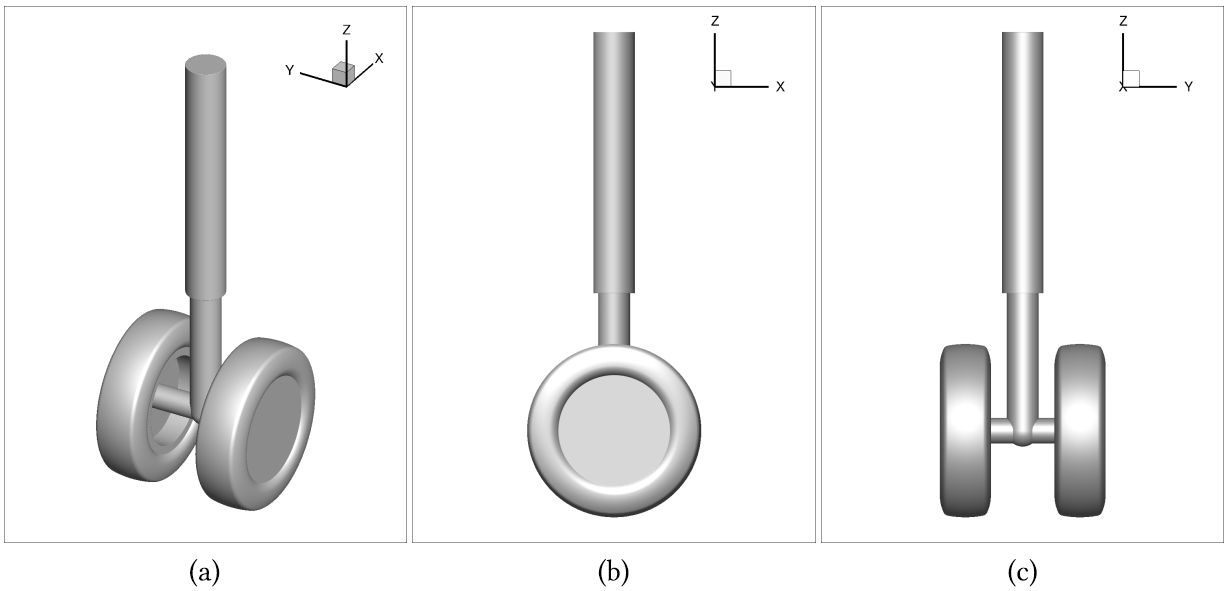
\includegraphics[width=0.9\columnwidth]{figures/landing_gear_model.png}
  \bicaption[不同视角下LAGOON起落架模型的示意图]{不同视角下LAGOON起落架模型的示意图。 (a) 等轴测投影; (b) $x-z$平面; (c) $y-z$平面。图片来自~\cite{doi:10.2514/6.2022-2850}。}{Schematics of the LAGOON landing gear at different views. (a) Isometric view; (b) $x-z$ plane; (c) $y-z$ plane. Image from~\cite{doi:10.2514/6.2022-2850}.}
  \label{img:landing_gear_model}
\end{figure}

本节对LAGOON模型进行初步的气动声学实验,以验证我们的方法在气动声学上依然可以满足工业标准的要求,所获得的不同方面的结果在下面列出。在实验中,我们设定的场景与CEPRA19风洞中进行实际风洞实验时的场景~\cite{doi:10.2514/6.2015-2993} 相同,即起落架模型置于0.23 Ma (78.99 $m/s$) 的气流中,起落架的直径$D=0.3m$,雷诺数$Re=1.541\times 10^6$。

我们首先展示一些流场的可视化。在图~\ref{img:landing_gear_pressure} 中我们展示起落架在$y=0$平面上的瞬时压力分布,图中清楚地显示出了在高速的流体中,起落架所造成的高压区与低压区。图~\ref{img:landing_gear_pressure} 中我们展示起落架在Q值为$1.0\times 10^6 s^{-2}$时的等值面。这些Q值的等值面显示涡度模值远大于应变速率模值的位置。从图中我们可以看到流体是高度不稳定的,且有很多小的湍流涡旋从起落架上激发。

\begin{figure}[!htbp]
  \centering
    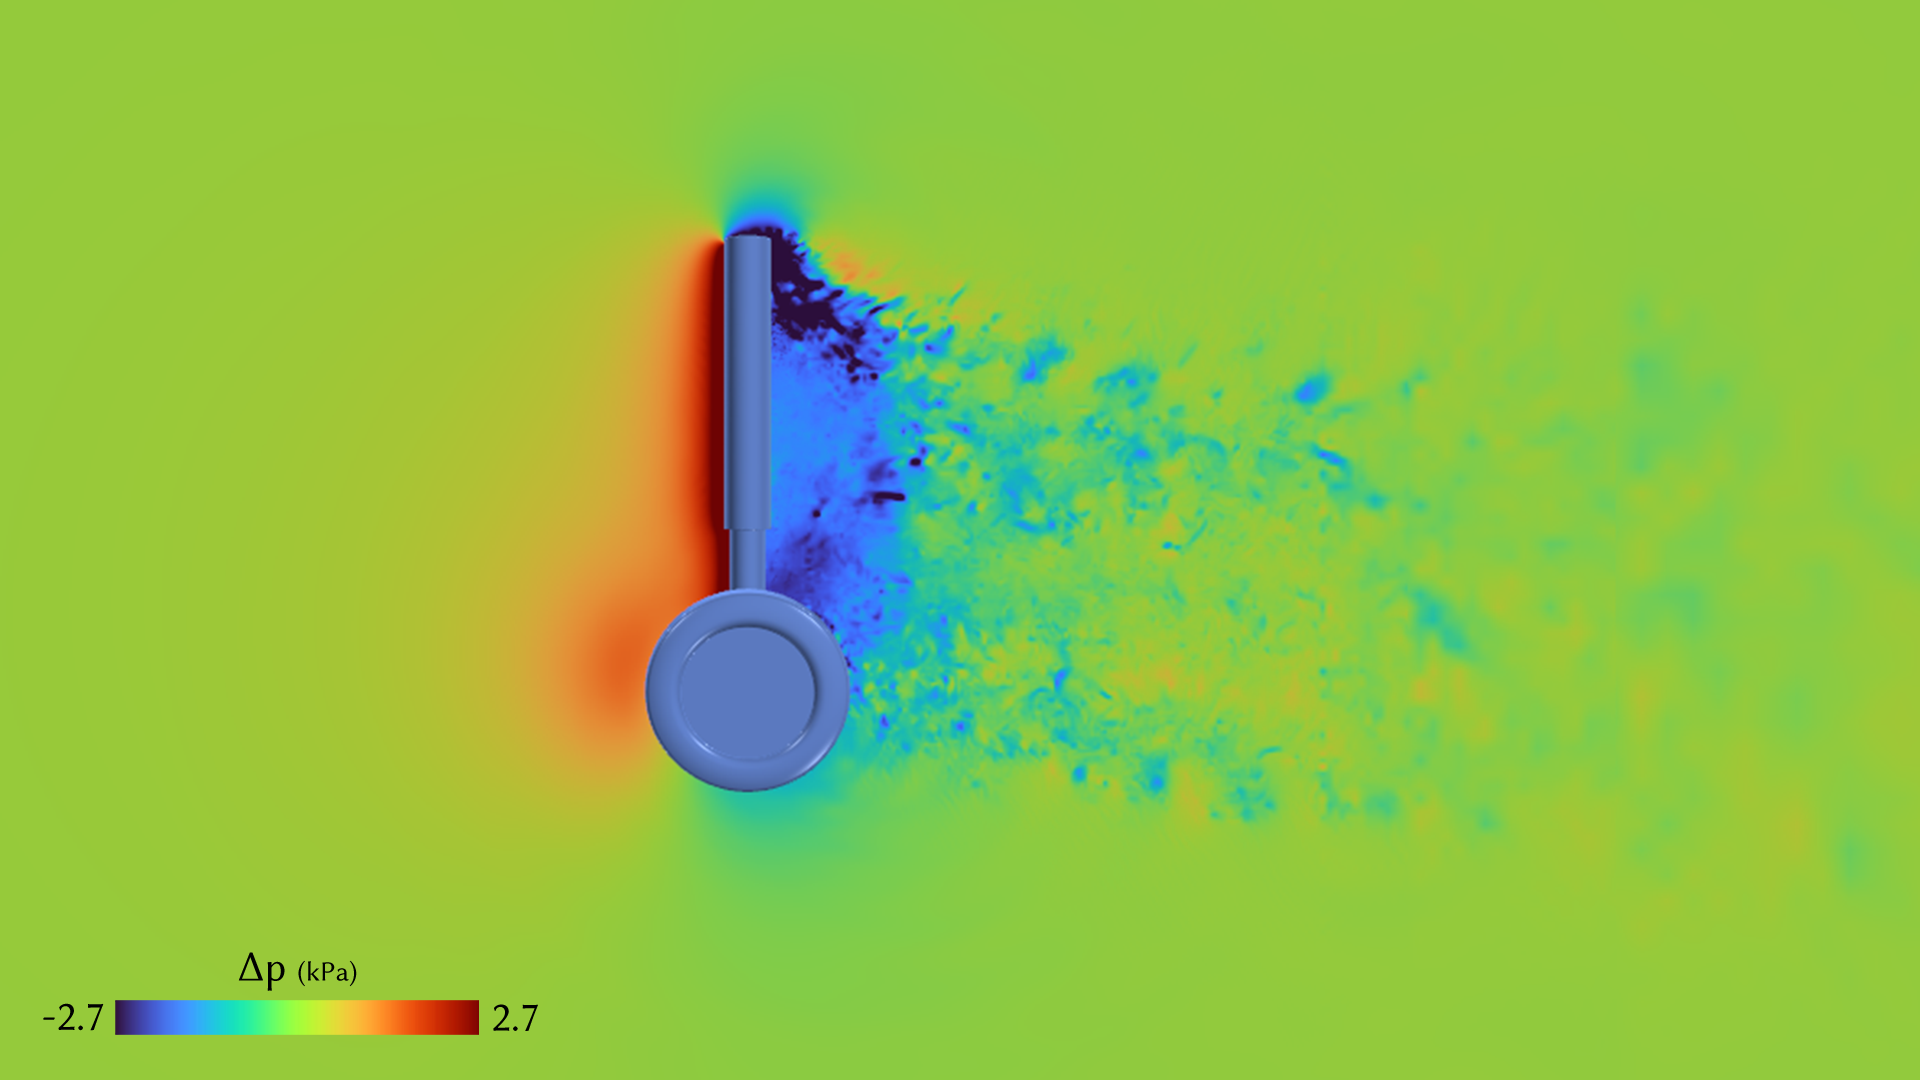
\includegraphics[width=0.99\columnwidth]{figures/landing_gear_pressure.png}
  \bicaption[LAGOON起落架在$y=0$平面上的瞬时压力分布]{LAGOON起落架在$y=0$平面上的瞬时压力分布。}{Instantaneous pressure distribution of LAGOON landing gear in the $y=0$ plane.}
  \label{img:landing_gear_pressure}
\end{figure}

\begin{figure}[!htbp]
  \centering
    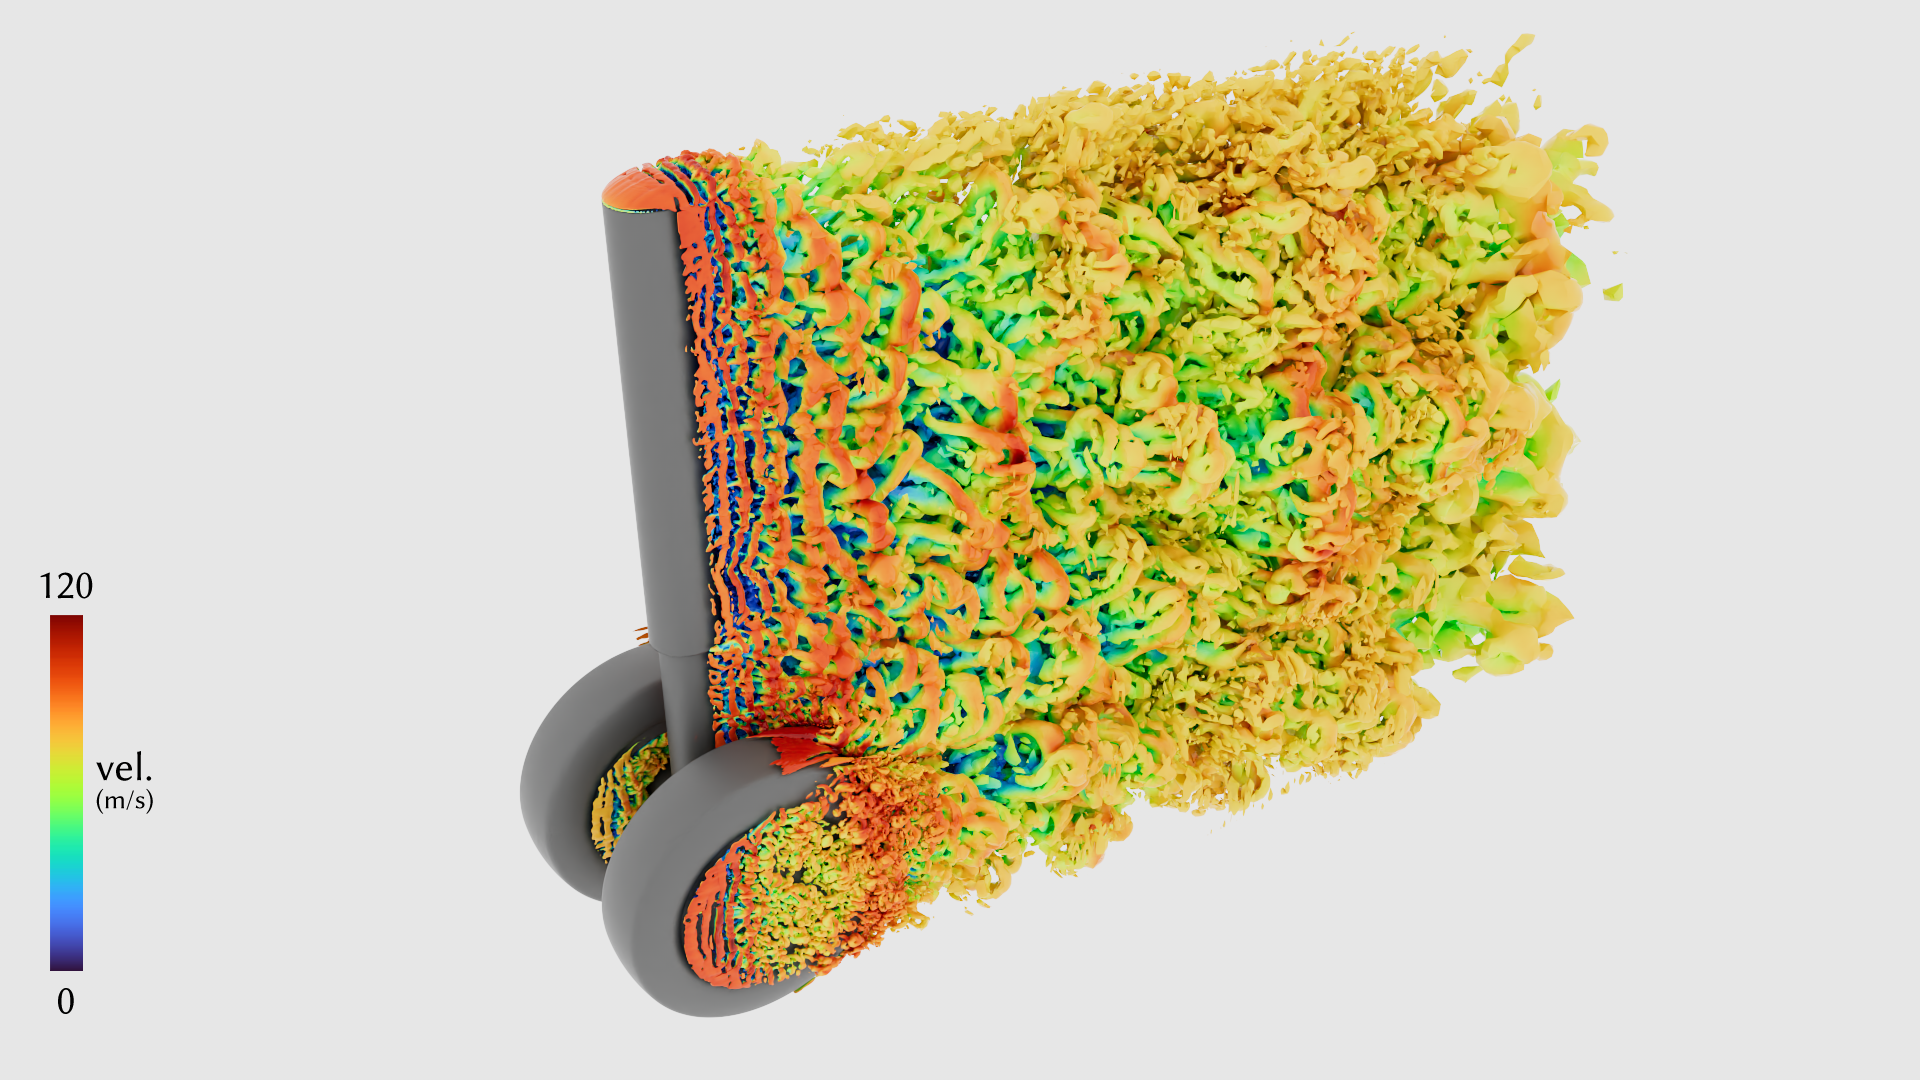
\includegraphics[width=0.99\columnwidth]{figures/landing_gear_q_criterion.png}
  \bicaption[LAGOON起落架在Q值为$1.0\times 10^6 s^{-2}$时的等值面]{LAGOON起落架在Q值为$1.0\times 10^6 s^{-2}$时的等值面。等值面的颜色来自瞬时速度的模值。}{Iso-surfaces of Q-criterion at the value of $1.0\times 10^6 s^{-2}$ of LAGOON landing gear. The iso-surfaces are colored by instantaneous velocity magnitude.}
  \label{img:landing_gear_q_criterion}
\end{figure}

我们接下来展示一些与声音更直接相关的可视化与数值结果。首先在图~\ref{img:landing_gear_divergence} 中我们展示起落架在$y=0$平面上的胀量场分布,以突出声波的分布。从图中我们可以看到两处很明显的声波扰动 (acoustic perturbation) 来源:一处是起落架轮胎的下部,一处是起落架撑杆的顶部。并且我们也可以看到在起落架撑杆的后方 (相对于来流方向),有很强的湍流对流 (turbulent convection)。为了进一步定性分析,我们在起落架模型的右轮胎上取一个采样点 (见图~\ref{img:landing_gear_frequency} (a)),并测量该点的压力变化。之后使用加窗平均周期图法 (Welch法~\cite{1161901}) 对压力序列进行处理以获得频谱,见过可见图~\ref{img:landing_gear_frequency} (b)。图中蓝色线条为我们测得的结果,红色线条为CEPRA19风洞中的实际实验结果~\cite{doi:10.2514/6.2015-2993}。结果显示我们可以成功预测在约$1000Hz$与$1500Hz$出现的声调,与实验相吻合。

\begin{figure}[!htbp]
  \centering
    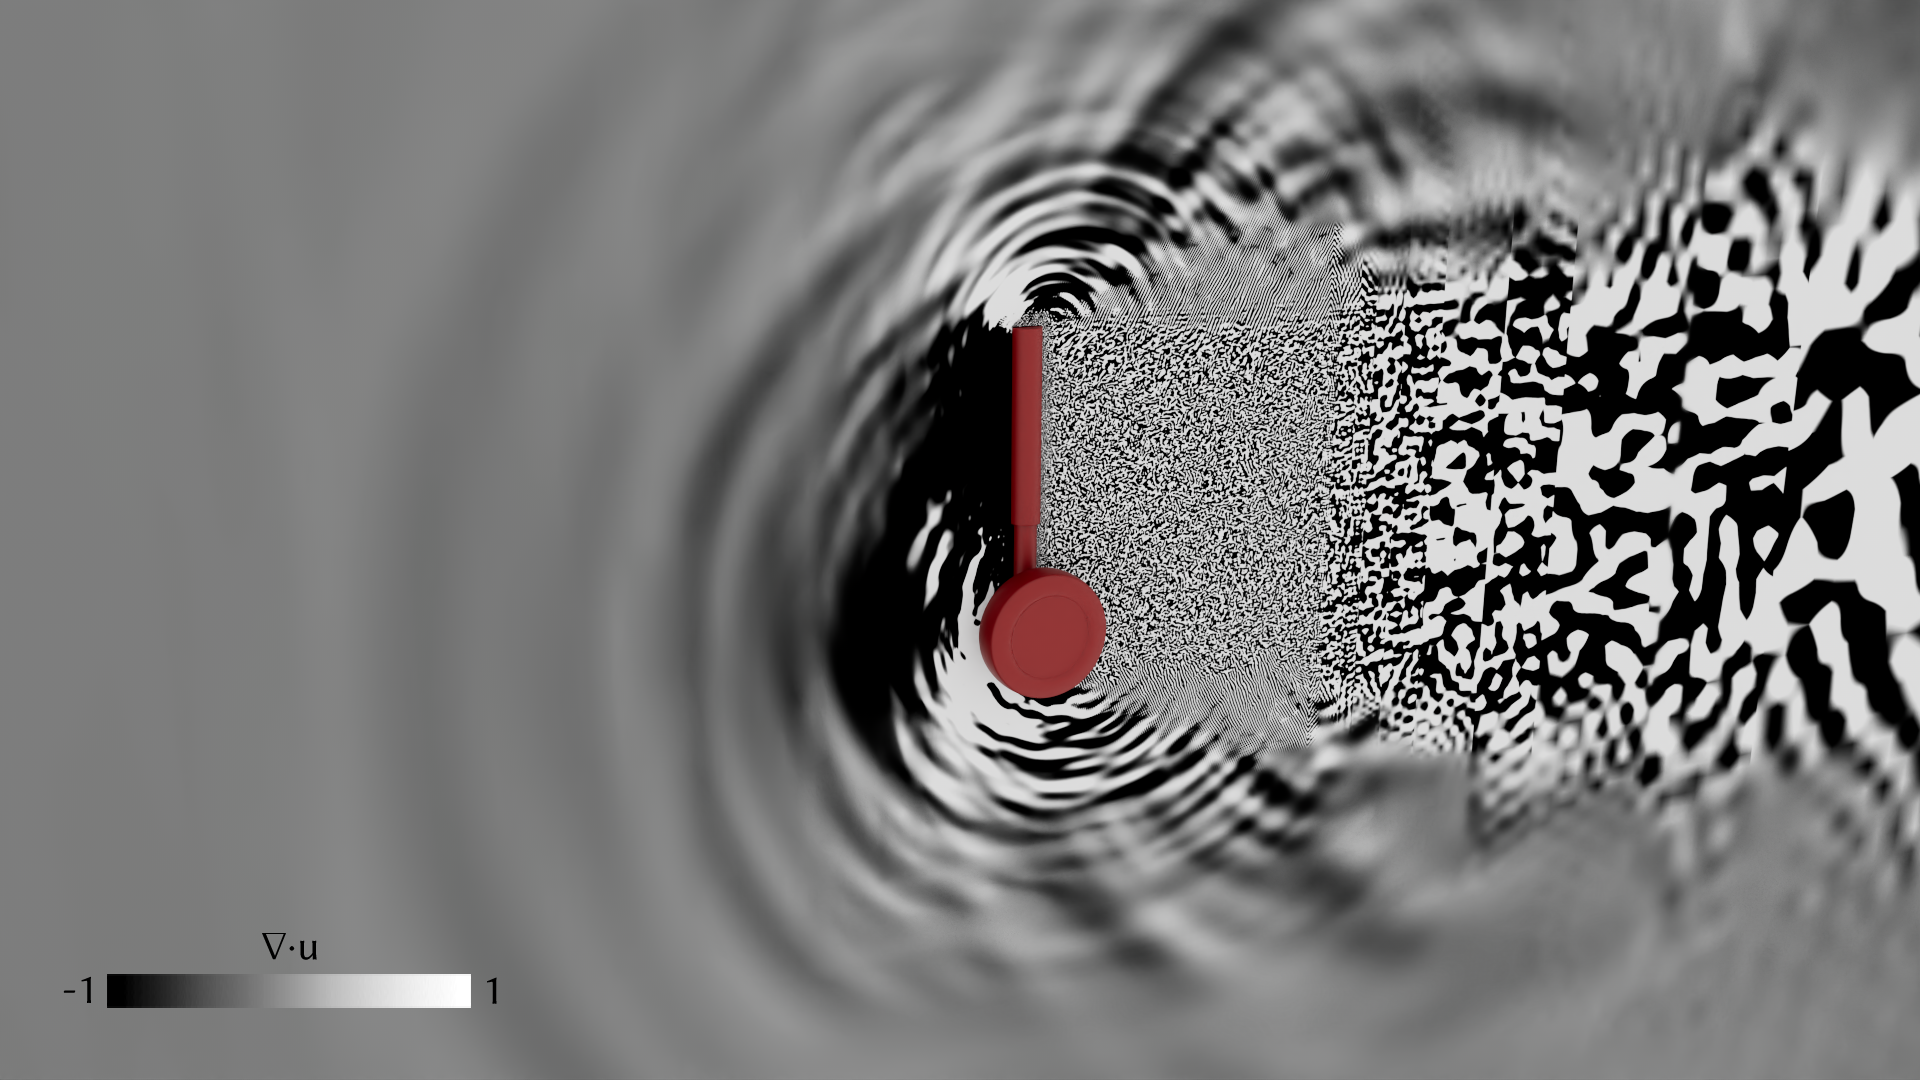
\includegraphics[width=0.99\columnwidth]{figures/landing_gear_divergence.png}
  \bicaption[LAGOON起落架在$y=0$平面上的胀量场分布(灰阶)]{LAGOON起落架在$y=0$平面上的胀量场分布(灰阶)。}{Dilatation field in the $y=0$ plane of LAGOON landing gear in grayscale.}
  \label{img:landing_gear_divergence}
\end{figure}

\begin{figure}[!htbp]
  \centering
    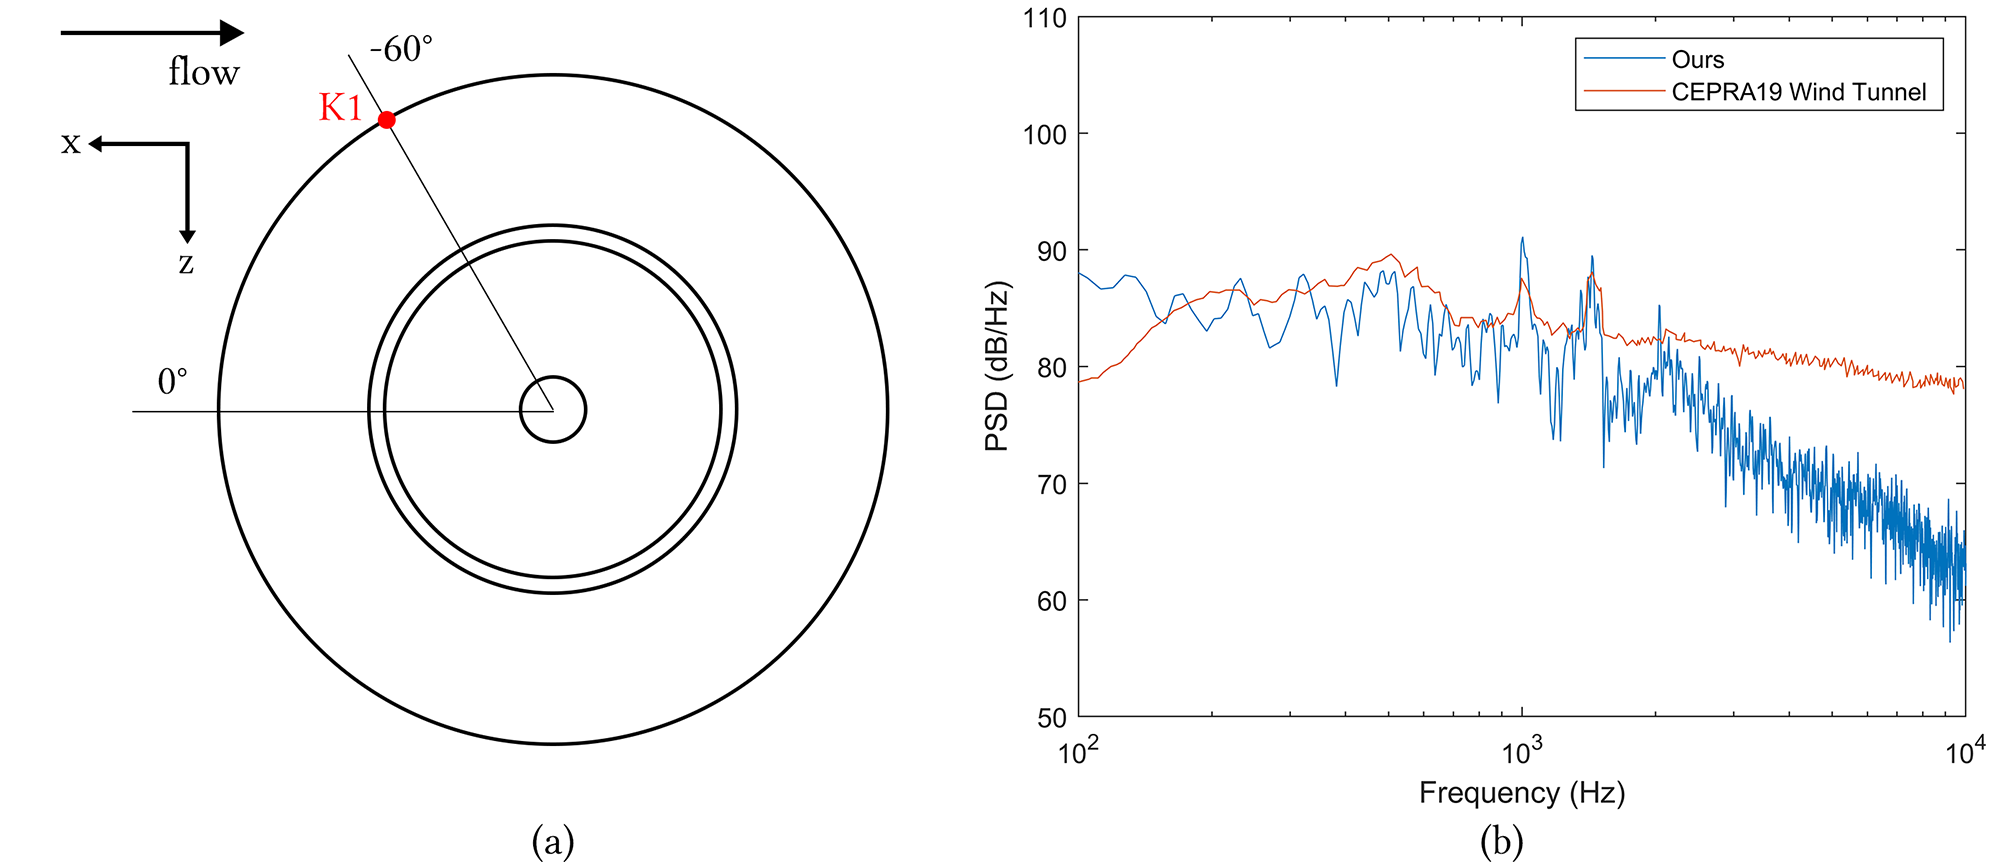
\includegraphics[width=0.99\columnwidth]{figures/landing_gear_frequency.png}
  \bicaption[LAGOON起落架轮胎采样点的功率谱密度]{LAGOON起落架轮胎采样点的功率谱密度。在右轮胎上的采样点K1 (a) 测得压力序列后进行信号分析,得到该点的功率谱密度 (b)。其中蓝色线条为我们测得的结果,红色线条为CEPRA19风洞中的实际实验结果~\cite{doi:10.2514/6.2015-2993}。结果显示我们可以成功预测在约$1000Hz$与$1500Hz$出现的声调,与实验相吻合。}{Power spectral density of a sample point on the LAGOON landing gear tire. We mearsure the pressure sequence from a sample point K1 on the right tire (a) and obtain its power spectral density via signal analysis (b). Blue curve shows our mearsurement and red curve shows the result from CEPRA19 wind tunnel testing. It demonstrates that we can successfully predict the tonal emergence at about $1000Hz$ and $1500Hz$, which matches the experiment.}
  \label{img:landing_gear_frequency}
\end{figure}